\documentclass[12pt,a4paper,oneside]{report}

\usepackage[utf8]{inputenc}
\usepackage[T1]{fontenc}
\usepackage[brazil]{babel}
\usepackage{microtype}
\usepackage{amsmath, amsfonts, amssymb}
\usepackage{graphicx}
\usepackage{booktabs}
\usepackage{multirow}
\usepackage{makecell}
\usepackage{xcolor}
\usepackage{listings}
\usepackage{hyperref}
\usepackage{tabularx}
\usepackage{float}
\usepackage{subcaption}
\usepackage[margin=2.5cm]{geometry}

% Inclusão do arquivo de configurações
% ==============================================================================
% CONFIGURAÇÕES DE PACOTES E CUSTOMIZAÇÕES (ABNTEX2)
% ==============================================================================

\usepackage[utf8]{inputenc}
\usepackage[T1]{fontenc}
\usepackage{microtype}
\usepackage{amsmath, amsfonts, amssymb}
\usepackage{graphicx}
\usepackage{booktabs}
\usepackage{multirow}
\usepackage{makecell}
\usepackage{xcolor}
\usepackage{listings}
\usepackage{hyperref}
\usepackage{tabularx}
\usepackage{float}
\usepackage{subcaption}

% Configurações de Cores
\definecolor{codegreen}{rgb}{0,0.6,0}
\definecolor{codegray}{rgb}{0.5,0.5,0.5}
\definecolor{codepurple}{rgb}{0.58,0,0.82}
\definecolor{backcolour}{rgb}{0.96,0.96,0.96}
\definecolor{darkblue}{rgb}{0.0,0.0,0.55}

% Estilo de Listings (Códigos)
\lstdefinestyle{mystyle}{
    backgroundcolor=\color{backcolour},   
    commentstyle=\color{codegreen},
    keywordstyle=\color{darkblue}\bfseries,
    numberstyle=\tiny\color{codegray},
    stringstyle=\color{codepurple},
    basicstyle=\ttfamily\footnotesize,
    breakatwhitespace=false,         
    breaklines=true,                 
    captionpos=b,                    
    keepspaces=true,                 
    numbers=left,                    
    numbersep=5pt,                  
    showspaces=false,                
    showstringspaces=false,
    showtabs=false,                  
    tabsize=2
}
\lstset{style=mystyle}

% Configuração de Links Hyperref
\hypersetup{
    colorlinks=true,
    linkcolor=darkblue,
    citecolor=darkblue,
    urlcolor=darkblue
}

% Comandos Matemáticos Customizados
\DeclareMathOperator*{\argmin}{arg\,min}
\DeclareMathOperator*{\argmax}{arg\,max}
\newcommand{\psnr}{\text{PSNR}}
\newcommand{\rmse}{\text{RMSE}}
\newcommand{\mae}{\text{MAE}}


\graphicspath{{Imagens/}}

\begin{document}

\begin{titlepage}
    \centering
    \vspace*{0.5cm}
    {\large \textbf{INSTITUTO FEDERAL DE EDUCAÇÃO, CIÊNCIA E TECNOLOGIA DE PERNAMBUCO}}\\[0.2cm]
    {\large \textbf{CAMPUS PAULISTA}}\\[0.2cm]
    {\large \textbf{CURSO SUPERIOR DE TECNOLOGIA EM ANÁLISE E DESENVOLVIMENTO DE SISTEMAS}}\\[3.0cm]
    
    {\Large \textbf{VICTOR GIULIANO DE FREITAS SILVA}}\\[2.5cm]
    
    {\LARGE \textbf{DIAGNÓSTICO FITOSSANITÁRIO EM FOLHAS DE CANA-DE-AÇÚCAR VIA CNN EMBARCADA COM TINYML, PIPELINE ASSÍNCRONO DUAL-CORE NO ESP32-S3 E CO-SIMULAÇÃO HIL COM VANT}}\\[3.0cm]
    
    \vfill
    {\large Paulista -- PE\\2026}
\end{titlepage}

% Folha de Rosto
\newpage
\thispagestyle{empty}
\begin{center}
    \vspace*{0.5cm}
    {\Large \textbf{VICTOR GIULIANO DE FREITAS SILVA}}\\[3.5cm]
    
    {\LARGE \textbf{DIAGNÓSTICO FITOSSANITÁRIO EM FOLHAS DE CANA-DE-AÇÚCAR VIA CNN EMBARCADA COM TINYML, PIPELINE ASSÍNCRONO DUAL-CORE NO ESP32-S3 E CO-SIMULAÇÃO HIL COM VANT}}\\[3.0cm]
    
    \hspace{.45\textwidth}
    \begin{minipage}{.5\textwidth}
        \small
        Trabalho de Conclusão de Curso apresentado ao Curso Superior de Tecnologia em Análise e Desenvolvimento de Sistemas do Instituto Federal de Educação, Ciência e Tecnologia de Pernambuco -- Campus Paulista, como requisito parcial para obtenção do título de Tecnólogo em Análise e Desenvolvimento de Sistemas.\\[0.8cm]
        \textbf{Orientador(a):} Prof(a). [Nome do Orientador]
    \end{minipage}
    
    \vfill
    {\large Paulista -- PE\\2026}
\end{center}

\newpage
\tableofcontents
\newpage

\chapter{Introdução}
\label{cap:introducao}

\section{Contextualização Histórica, Socioeconômica e Relevância Agronômica}

A cultura da cana-de-açúcar (\textit{Saccharum officinarum} L.) constitui um dos pilares históricos, econômicos e socioculturais mais profundos do Brasil e, em particular, do estado de Pernambuco. Desde o período colonial, com a implantação dos primeiros engenhos nas Capitanias Hereditárias no século XVI, a capitania de Pernambuco destacou-se como o polo açucareiro mais próspero da colônia, impulsionando a ocupação demográfica e territorial do litoral e da Zona da Mata nordestina \cite{freyre2004}. Conforme documentado pela historiografia clássica brasileira \cite{freyre2004,mello2007}, a economia canavieira forjou a estrutura social, a dinâmica política e a fisionomia agrária regional por mais de quatro séculos.

Na contemporaneidade, a despeito da industrialização e diversificação econômica do estado, a cana-de-açúcar preserva centralidade vital na matriz produtiva regional. Dados consolidados da Companhia Nacional de Abastecimento \cite{conab2024cana,conab2025} e do Sindicato da Indústria do Açúcar e do Álcool no Estado de Pernambuco \cite{sindacucar2024} atestam que o estado processou aproximadamente 11,6 milhões de toneladas de cana na safra recente, respondendo por parcela substancial do Produto Interno Bruto (PIB) agropecuário nordestino, fornecendo matéria-prima para a produção de açúcar, etanol carburante e bioeletricidade limpa, além de sustentar cerca de 70 mil empregos diretos \cite{santos2023}. Ademais, a cadeia produtiva da cana em Pernambuco abrange milhares de pequenos fornecedores e famílias assentadas na Zona da Mata que dependem economicamente da sanidade de seus canaviais, configurando um ecossistema com forte relevância para a agricultura familiar \cite{oliveira2024}.

Entretanto, a rentabilidade do setor sucroenergético e a subsistência do pequeno produtor enfrentam contínuas perdas agronômicas decorrentes de pragas e fitopatologias foliares de alta transmissibilidade \cite{mariano2023}. Dentre os patógenos mais devastadores que acometem os canaviais tropicais, destacam-se o Carvão (\textit{Sporisorium scitamineum}), a Ferrugem Marrom (\textit{Puccinia melanocephala}), o Complexo de \textit{Fusarium} (\textit{Pokkah Boeng}), a Mancha Parda (\textit{Cercospora longipes}), a Podridão de Toletes (\textit{Ceratocystis paradoxa}), a Podridão Vermelha (\textit{Colletotrichum falcatum}) e viroses sistêmicas como a Síndrome da Folha Amarela (SCYLV) e o Mosaico \cite{barbedo2019review}. Essas enfermidades induzem clorose, necroses vasculares nos colmos e quebra drástica no rendimento de sacarose, provocando perdas produtivas de 20\% a 50\% quando não identificadas precocemente \cite{mariano2023,conab2025}.

A contenção fitossanitária eficaz repousa na intervenção localizada (*Precision Spraying*) antes da dispersão das teliósporos e conídios. Contudo, o método tradicional dominante ainda consiste no caminhamento técnico pedestre por pragueiros (*scouting* manual). Diante do porte denso e cortante da cana adulta (frequentemente superando três metros de altura) e de talhões que ultrapassam centenas de hectares contínuos, a inspeção manual é morosa, excessivamente onerosa, subjetiva e incapaz de monitorar a totalidade das lavouras em tempo hábil \cite{radoglou2020compilation}.

\section{A Problemática Tecnológica: Conectividade Rural vs. IA em Nuvem}

O recente avanço do Aprendizado Profundo (*Deep Learning*) e das Redes Neurais Convolucionais (*Convolutional Neural Networks* -- CNNs) viabilizou o diagnóstico automatizado de patologias vegetais a partir de fotos RGB com alta sensibilidade \cite{krizhevsky2012,lu2022}. Todavia, a esmagadora maioria das abordagens disponíveis na literatura acadêmica baseia-se no paradigma da Computação em Nuvem (*Cloud Computing*), no qual imagens adquiridas em campo são enviadas continuamente para servidores remotos providos de placas gráficas de alto custo (GPUs) \cite{xu2023,rodriguez2021sugarcane}.

No contexto da agricultura brasileira e, em particular, na Zona da Mata pernambucana, a dependência da nuvem esbarra em barreiras intransponíveis:
\begin{enumerate}
    \item \textbf{Ausência de Conectividade Rural:} Grandes porções das zonas rurais sofrem com sombra de sinal de telefonia celular 3G/4G, inviabilizando o upload contínuo de fluxos de vídeo ou pacotes massivos de fotos de alta resolução durante a jornada de inspeção \cite{he2023};
    \item \textbf{Latência de Enlace e Incerteza Operacional:} A oscilação dos enlaces sem fio rurais impõe latências imprevisíveis de vários segundos por foto, inviabilizando tomadas de decisão imediatas em controle de voo ou prescrição em tempo real;
    \item \textbf{Custo de Aceleradores Dedicados:} Computadores de bordo industriais baseados em GPU (como a família NVIDIA Jetson) apresentam custo elevado, peso excessivo e consumo energético incompatível com a realidade orçamentária da agricultura familiar e com aeronaves não tripuladas leves \cite{oliveira2024}.
\end{enumerate}

Como alternativa, a disciplina de *Tiny Machine Learning* (*TinyML*) \cite{warden2019,moons2020} viabilizou a execução de redes neurais profundas inteiramente quantizadas diretamente em microcontroladores de baixo custo ($< \text{US\$} 5$) e consumo na faixa de miliwatts, como o SoC Espressif ESP32-S3 \cite{esp32s3}. Ao transferir a inferência matemática para a borda extrema (*Extreme Edge*), elimina-se integralmente a dependência de conectividade externa, garantindo autonomia, determinismo temporal e preservação dos dados.

\section{A Integração de TinyML com Veículos Aéreos Não Tripulados via MAVLink}

Paralelamente, o emprego de Veículos Aéreos Não Tripulados (VANTs), ou drones, revolucionou o sensoriamento remoto agrícola ao conferir elevada mobilidade espacial para inspeção sobre a copa dos canaviais \cite{radoglou2020compilation}.

Entretanto, as abordagens convencionais com drones limitam-se ao processamento estático pós-voo: o VANT sobrevoa a plantação registrando fotos indiscriminadamente em cartões de memória para posterior fotogrametria manual em escritório, horas após o pouso. Ademais, aeronaves em voo contínuo acopladas a sensores ópticos de baixo custo com obturador eletrônico por rolamento (*rolling shutter*) sofrem severo borrão de movimento (*motion blur*) decorrente da velocidade de translação e das vibrações mecânicas, degradando as feições microscópicas das lesões foliares.

Nesse contexto, surge a oportunidade científica de integrar o microcontrolador ESP32-S3 como um computador de bordo inteligente (*Companion Payload*) acoplado ao piloto automático do drone via protocolo aeroespacial padrão **MAVLink v2** \cite{koubaa2019mavlink}. Em vez de atuar como mero espectador passivo, o microcontrolador executa uma máquina de estados autônoma de **Parada Amostral Sistemática (*Pause-and-Classify*)**: comanda a aeronave a pairar (*hover*) nos waypoints da grade de plantio, aguarda a dissipação de vibrações ($500\text{ ms}$), captura e processa a imagem foliar on-chip em alta resolução, registra a predição sincronizada com a telemetria GPS e libera o voo para o próximo ponto, sintetizando mapas de calor pós-missão para Sistemas de Informação Geográfica (SIG).

\section{Objetivos}

\subsection{Objetivo Geral}

O objetivo geral deste trabalho é projetar, implementar, otimizar e validar experimentalmente um sistema inteligente, autônomo e de baixo custo para avaliação fitossanitária de 11 classes foliares de cana-de-açúcar, composto por uma rede neural convolucional quantizada em inteiros de 8 bits (\textit{INT8}) embarcada no microcontrolador dual-core ESP32-S3, integrada a uma estratégia de controle de VANT via protocolo MAVLink sob o paradigma de Parada Amostral Sistemática (\textit{Pause-and-Classify}).

\subsection{Objetivos Específicos}

Para consecução do objetivo geral, estabelecem-se os seguintes objetivos específicos:
\begin{enumerate}
    \item Executar uma auditoria forense criptográfica rigorosa baseada em hashes MD5 sobre as 6.748 imagens do *Sugarcane Leaf Image Dataset*, identificando e expurgando duplicatas internas e 614 arquivos envolvidos em colisões cruzadas de rótulos entre classes incompatíveis (notadamente entre *smut* e *Pokkah Boeng*);
    \item Desenvolver e treinar o modelo neural MobileNetV2 ($\alpha=0,75$, entrada $160 \times 160$) com Perda Focal Categórica e quantização inteira completa INT8 (\texttt{v08}), superando o colapso diagnóstico da classe Carvão;
    \item Formular, modelar matematicamente e implementar no firmware C++ o algoritmo de pré-processamento **Modo 7 (RGB8888 + Box-Averaging com LUT Q16 e escala IDCT)**, eliminando o viés DC de escurecimento e garantindo paridade radiométrica exata ($\text{PSNR} = \infty\text{ dB}$);
    \item Projetar uma arquitetura de paralelismo híbrido em dois níveis no FreeRTOS (pipeline assíncrono inter-quadros e *Fork-Join* intra-inferência com alocação de $48\text{ KB}$ de *scratch buffer* na SRAM interna), mitigando a contenção na Octal PSRAM e acelerando as convoluções via instruções vetoriais SIMD Xtensa LX7;
    \item Avaliar exaustivamente o sistema no hardware físico sobre **9.269 imagens**, mensurando latência, vazão e diagnosticando empiricamente o fenômeno de Deslocamento de Domínio (*Domain Shift*) frente a sensores heterogêneos;
    \item Construir e validar a bancada de Co-Simulação *Hardware-in-the-Loop* (HIL) MAVLink em malha fechada sobre um talhão agrícola de 55 waypoints, sintetizando automaticamente camadas vetoriais GeoJSON (RFC 7946) e mapas de calor de focos epidêmicos compatíveis com QGIS.
\end{enumerate}

\section{Estrutura do Trabalho}

Esta monografia está estruturada em cinco capítulos:
\begin{itemize}
    \item \textbf{Capítulo \ref{cap:fundamentacao}}: Apresenta a fundamentação teórica sobre fitopatologia da cana, redes convolucionais leves (MobileNetV2), quantização inteira simétrica INT8, extensões vetoriais SIMD no ESP32-S3, teoria de amostragem de Nyquist-Shannon e protocolo MAVLink;
    \item \textbf{Capítulo \ref{cap:metodologia}}: Descreve a metodologia de engenharia, compreendendo a auditoria MD5 do dataset, o algoritmo de pré-processamento Modo 7, a arquitetura paralela FreeRTOS e a bancada HIL MAVLink;
    \item \textbf{Capítulo \ref{cap:resultados}}: Expõe e discute os resultados experimentais obtidos diretamente no hardware físico, incluindo benchmarks radiométricos, desempenho multinúcleo, avaliação massiva de 9.269 amostras com análise de *Domain Shift* e a missão HIL georreferenciada;
    \item \textbf{Capítulo \ref{cap:conclusao}}: Sintetiza as conclusões, avalia o impacto na agricultura familiar e delineia os trabalhos futuros.
\end{itemize}

\chapter{Fundamentação Teórica}
\label{cap:fundamentacao}

Este capítulo estabelece os alicerces teóricos e matemáticos que sustentam a presente pesquisa, cobrindo a fitopatologia da cana-de-açúcar, arquiteturas convolucionais eficientes, a teoria de quantização afim em inteiros de 8 bits, o processamento de sinais e amostragem na conversão de imagens, a arquitetura de hardware do processador ESP32-S3 e o protocolo aeroespacial MAVLink.

\section{Fitopatologia da Cana-de-Açúcar}

A cana-de-açúcar (\textit{Saccharum officinarum}) é suscetível a uma vasta gama de infecções que afetam a estrutura morfológica e a taxa fotossintética do dossel vegetativo. A caracterização botânica e sintomatológica das 11 classes avaliadas neste trabalho é descrita a seguir:

\begin{enumerate}
    \item \textbf{Carvão da Cana (\textit{smut} — \textit{Sporisorium scitamineum}):} Uma das doenças fúngicas mais graves do mundo. O sintoma patognomônico é a emergência de uma estrutura cilíndrica e chicoteada na gema apical da planta (o ``chicote''), recoberta inicialmente por uma membrana prateada que se rompe liberando bilhões de teliósporos marrom-escuros. Causa deformação total das folhas, afinamento dos colmos e perdas de até 100\% em variedades suscetíveis.
    \item \textbf{Pokkah Boeng (\textit{Fusarium moniliforme} / \textit{Gibberella fujikuroi}):} Patologia caracterizada pelo enrugamento, clorose basal e deformação retorcida das folhas apicais jovens (efeito ``folha amassada''). Em estágios avançados, o fungo penetra o meristema terminal provocando a podridão do topo da planta e morte do colmo.
    \item \textbf{Ferrugem Marrom (\textit{BrownRust} — \textit{Puccinia melanocephala}):} Manifesta-se inicialmente por pequenas pontuações cloróticas amareladas visíveis em ambas as faces da folha, que evoluem para pústulas alongadas de coloração marrom-avermelhada paralelas às nervuras. O rompimento da epiderme foliar acelera a dessecação e desfolha precoce.
    \item \textbf{Mancha Parda (\textit{Brown Spot} — \textit{Cercospora longipes}):} Lesões circulares a ovais de bordas bem delimitadas marrom-escuras com centro avermelhado ou cinza, amplamente disseminadas nas folhas medianas e velhas sob condições de alta umidade.
    \item \textbf{Clorose Zonada (\textit{Banded Chlorosis}):} Distúrbio fisiológico induzido por estresses térmicos bruscos (ondas repentinas de frio no início do desenvolvimento), caracterizado por faixas horizontais esbranquiçadas ou cloróticas transversais ao longo de todo o limbo foliar.
    \item \textbf{Síndrome da Folha Amarela (\textit{Yellow Leaf} — \textit{Sugarcane Yellow Leaf Virus} - SCYLV):} Vírus transmitido por pulgões que induz amarelecimento intenso e progressivo da nervura central das folhas intermediárias em direção às margens, inibindo o acúmulo de sacarose e reduzindo o peso do colmo.
    \item \textbf{Viroses Foliares (\textit{Viral Disease} — Mosaico / \textit{Sugarcane Mosaic Virus}):} Induzem a formação de manchas cloróticas irregulares dispersas em padrão de ilhas verdes escuras contra fundo verde-claro no tecido foliar jovem.
    \item \textbf{Brotamento Graminoso (\textit{Grassy shoot} — Fitoplasma):} Proliferação desordenada e hipertrofiada de perfilhos finos, cloróticos e desprovidos de colmo aproveitável na base da touceira, conferindo à planta aspecto cespitoso semelhante a uma gramínea.
    \item \textbf{Podridão Abacaxi do Colmo (\textit{Sett Rot} — \textit{Ceratocystis paradoxa}):} Infecção que acomete prioritariamente os toletes de plantio e a base dos colmos, provocando avermelhamento interno do parênquima com odor aromático frutado característico de ésteres de abacaxi, culminando na podridão negra dos tecidos.
    \item \textbf{Folhas Secas (\textit{Dried Leaves}):} Senescência avançada e perda completa de turgor celular associada a estresse hídrico severo ou ataques fúngicos terminais.
    \item \textbf{Folhas Sadias (\textit{Healthy Leaves}):} Tecido foliar íntegro, com pigmentação verde homogênea e ausência de lesões necróticas ou cloróticas.
\end{enumerate}

\section{Redes Convolucionais e Arquiteturas Leves (MobileNets)}

As Redes Neurais Convolucionais tradicionais processam tensores tridimensionais de entrada $X \in \mathbb{R}^{H \times W \times C_{in}}$ através de camadas convolucionais densas compostas por $C_{out}$ filtros de dimensões $K \times K \times C_{in}$. O custo computacional medido em operações de multiplicação e acumulação (\textit{Multiply-Accumulate} - MACs) de uma convolução padrão é expresso por:
\begin{equation}
\text{Custo}_{\text{Padrão}} = H \cdot W \cdot C_{in} \cdot C_{out} \cdot K^2
\label{eq:custo_conv_padrao}
\end{equation}

Para microcontroladores de borda dotados de pouca memória e sem aceleradores gráficos, esse custo computacional é proibitivo. A família de arquiteturas MobileNet \cite{howard2017mobilenets, sandler2018mobilenetv2} solucionou esse gargalo fatorando a convolução padrão em duas operações especializadas: a \textbf{Convolução em Profundidade} (\textit{Depthwise Convolution}) e a \textbf{Convolução Pontual} (\textit{Pointwise Convolution $1\times1$}), denominadas conjuntamente como \textbf{Convoluções Separáveis em Profundidade} (\textit{Depthwise Separable Convolutions}):

\begin{enumerate}
    \item \textbf{Depthwise Convolution ($K \times K$):} Aplica um filtro espacial bidimensional independente a cada canal de entrada, gerando $C_{in}$ mapas intermediários:
    \begin{equation}
    \text{Custo}_{\text{Depthwise}} = H \cdot W \cdot C_{in} \cdot K^2
    \end{equation}
    \item \textbf{Pointwise Convolution ($1 \times 1$):} Realiza uma combinação linear estritamente entre canais ao longo de cada posição espacial para sintetizar as $C_{out}$ características de saída:
    \begin{equation}
    \text{Custo}_{\text{Pointwise}} = H \cdot W \cdot C_{in} \cdot C_{out} \cdot 1^2
    \end{equation}
\end{enumerate}

A soma dessas duas etapas define o custo total da convolução separável:
\begin{equation}
\text{Custo}_{\text{Separável}} = H \cdot W \cdot C_{in} \cdot K^2 + H \cdot W \cdot C_{in} \cdot C_{out}
\label{eq:custo_separavel}
\end{equation}

Dividindo a Equação \ref{eq:custo_separavel} pela Equação \ref{eq:custo_conv_padrao}, obtém-se a razão exata de redução de esforço computacional:
\begin{equation}
\frac{\text{Custo}_{\text{Separável}}}{\text{Custo}_{\text{Padrão}}} = \frac{H \cdot W \cdot C_{in} \cdot (K^2 + C_{out})}{H \cdot W \cdot C_{in} \cdot C_{out} \cdot K^2} = \frac{1}{C_{out}} + \frac{1}{K^2}
\label{eq:razao_mobilenet}
\end{equation}
Para um filtro convencional de $K = 3$ e camadas típicas onde $C_{out} \gg 9$, a razão aproxima-se de $\frac{1}{9} \approx 0,111$. Isso representa uma \textbf{redução de cerca de 88\% a 90\% no volume de cálculos}, tornando a execução viável em frequências de clock de microcontroladores.

A versão MobileNetV2 introduziu ainda os blocos de \textbf{Resíduos Invertidos com Gargalos Lineares} (\textit{Inverted Residuals with Linear Bottlenecks}) \cite{sandler2018mobilenetv2}. Diferente das redes ResNet clássicas que comprimem os canais antes da convolução espacial, os blocos invertidos expandem as características para uma dimensão intermediária maior via projeção $1\times1$, executam a convolução espacial leve em profundidade e projetam novamente para um gargalo linear estrito de baixa dimensão sem ativação não-linear no ponto de soma residual, preservando a variedade geométrica (\textit{manifold}) das características latentes.

\section{Teoria da Quantização Afim Inteira (INT8)}
\label{sec:quantizacao_int8}

A representação de pesos e ativações em precisão de ponto flutuante de 32 bits (\textit{float32}) exige 4 bytes por parâmetro e demanda unidades de ponto flutuante (FPUs) pesadas. A quantização uniforme afim \cite{jacob2018quantization} mapeia tensores contínuos reais $r \in [\alpha, \beta]$ para inteiros com sinal de 8 bits $q \in [-128, 127]$ através da transformação matemática:
\begin{equation}
q = \text{clip}\left( \text{round}\left( \frac{r}{S} \right) + Z,\; q_{\min},\; q_{\max} \right)
\label{eq:quantizacao_direta}
\end{equation}
onde:
\begin{itemize}
    \item $S \in \mathbb{R}^+$ representa o fator de escala (\textit{scale factor}), que indica o valor real representado por uma unidade do inteiro quantizado;
    \item $Z \in \mathbb{Z}$ é o ponto zero (\textit{zero-point}), inteiro exato que mapeia o zero real ($r = 0.0$), garantindo que paddings nulos não sofram distorção numérica;
    \item $q_{\min} = -128$ e $q_{\max} = 127$ são os limites numéricos do tipo \texttt{int8\_t}.
\end{itemize}

A reconstrução aproximada (desquantização) do número real original é dada por:
\begin{equation}
r \approx S \cdot (q - Z)
\label{eq:desquantizacao}
\end{equation}

Em uma camada convolucional totalmente quantizada onde as ativações de entrada são denotadas por $q_1$, os pesos do filtro por $q_2$ e a saída por $q_3$, a multiplicação tensorial no domínio real $r_3 = r_1 \cdot r_2$ é transcrita para o domínio inteiro como:
\begin{equation}
S_3 \cdot (q_3 - Z_3) = \sum_{k} \Big[ S_1 \cdot (q_1^{(k)} - Z_1) \Big] \cdot \Big[ S_2^{(k)} \cdot (q_2^{(k)} - Z_2) \Big]
\end{equation}
Isolando a saída quantizada $q_3$:
\begin{equation}
q_3 = Z_3 + \left( \frac{S_1 \cdot S_2}{S_3} \right) \cdot \sum_{k} (q_1^{(k)} - Z_1)(q_2^{(k)} - Z_2)
\label{eq:matriz_quantizada}
\end{equation}

A constante de escala composta $M = \frac{S_1 \cdot S_2}{S_3} \in (0, 1)$ é decomposta computacionalmente em uma multiplicação inteira de 32 bits com multiplicador normalizado $M_0 \in [0.5, 1.0)$ e um deslocamento de bits à direita (*bit-shift*):
\begin{equation}
M = 2^{-n} \cdot M_0
\end{equation}

Essa propriedade formalizada por Jacob et al. \cite{jacob2018quantization} garante que \textbf{100\% do laço interno de convolução e acumulação matricial seja executado utilizando exclusivamente acumuladores inteiros de 32 bits e registradores de 8 bits}, sem invocar nenhuma instrução de ponto flutuante em tempo de execução.

\section{Processamento Digital de Sinais e Teoria de Amostragem na Decodificação de Imagem}

\subsection{Espaços de Cor e Viés DC na Conversão RGB565}

Em sistemas embarcados convencionais dotados de decodificadores JPEG, o bitstream Huffman YCbCr é frequentemente convertido para o espaço de cor reduzido \textbf{RGB565} (16 bits por pixel: 5 bits para Vermelho, 6 bits para Verde e 5 bits para Azul), visando economizar largura de banda para displays LCD. Para alimentar redes neurais que operam com 8 bits por canal ($[0, 255]$), os programadores comumente aplicam um preenchimento por zeros à direita (*Zero-Fill*):
\begin{align}
r_8 &= r_5 \ll 3 = r_5 \times 8 \label{eq:zerofill_r} \\
g_8 &= g_6 \ll 2 = g_6 \times 4 \label{eq:zerofill_g} \\
b_8 &= b_5 \ll 3 = b_5 \times 8 \label{eq:zerofill_b}
\end{align}

Demonstra-se matematicamente que esse procedimento introduz duas distorções severas:
\begin{enumerate}
    \item \textbf{Perda de Alcance Dinâmico:} O valor máximo alcançável para $r_8$ e $b_8$ é $31 \times 8 = 248$, enquanto para $g_8$ é $63 \times 4 = 252$. O branco puro ($255$) torna-se fisicamente inatingível.
    \item \textbf{Viés DC Negativo Sistemático (*Brightness Bias*):} Sob a hipótese de distribuição uniforme dos bits menos significativos truncados $k \in \{0, \dots, 2^{8-B}-1\}$, o erro esperado de amostragem é dado por:
    \begin{equation}
    E[\epsilon] = -\frac{1}{2^{8-B}} \sum_{k=0}^{2^{8-B}-1} k = -\frac{2^{8-B}-1}{2}
    \label{eq:bias_teorico}
    \end{equation}
    Para os canais de 5 bits ($B=5$, $2^{8-5}-1 = 7$):
    \begin{equation}
    \text{Bias}_{R} = \text{Bias}_{B} = -\frac{7}{2} = -3,50\text{ LSB}
    \end{equation}
    Para o canal de 6 bits ($B=6$, $2^{8-6}-1 = 3$):
    \begin{equation}
    \text{Bias}_{G} = -\frac{3}{2} = -1,50\text{ LSB}
    \end{equation}
    O viés DC médio esperado para imagens RGB é:
    \begin{equation}
    \text{Bias}_{\text{médio}} = \frac{-3,50 + (-1,50) + (-3,50)}{3} = -\mathbf{2,833\text{ LSB}}
    \end{equation}
    Esse deslocamento negativo atenua sistematicamente os pixels de toda a imagem, escurecendo folhas verdes e degradando padrões de contraste foliar.
\end{enumerate}

\subsection{Teorema de Nyquist-Shannon e Aliasing Espacial}

O Teorema da Amostragem de Nyquist-Shannon \cite{nyquist1928certain, shannon1949communication} estabelece que um sinal bidimensional contínuo $f(x, y)$ com frequência espacial máxima $(u_{\max}, v_{\max})$ só pode ser perfeitamente reconstruído sem distorção se a frequência de amostragem satisfizer:
\begin{equation}
f_{s, x} \ge 2 u_{\max}, \quad f_{s, y} \ge 2 v_{\max}
\end{equation}

Ao reduzir a resolução espacial de uma imagem de entrada de dimensões $W_{orig} \times H_{orig}$ ($768 \times 1024$) para o tensor de entrada da CNN de dimensões $W_{dst} \times H_{dst}$ ($160 \times 160$), a taxa de decimação é de aproximadamente $4,8 \times 6,4 \approx 30,72$ pixels por elemento de destino. 

Se o processo de subamostragem for implementado por decimação ingênua (amostragem pontual por sobrescrita ou vizinho mais próximo), as frequências espaciais superiores à frequência de Nyquist da grade de destino sofrem rebatimento espectral (*aliasing*), projetando componentes espaciais de alta frequência sobre as baixas frequências \cite{gonzalez2018digital}. Fisicamente, lesões finas de esporos fúngicos com espessura de 1 a 3 pixels na imagem original desaparecem ou assumem formatos geométricos artificiais.

Para cumprir o critério de Nyquist, deve-se aplicar previamente um filtro passa-baixas anti-aliasing sobre cada bloco de decimação antes de realizar a amostragem. No contexto computacional discreto de imagens, o integrador ideal de área é a Média de Caixa (*Box Averaging*):
\begin{equation}
I_{dst}(x', y') = \frac{1}{|\Omega(x', y')|} \sum_{(x, y) \in \Omega(x', y')} I_{orig}(x, y)
\label{eq:box_averaging}
\end{equation}
onde $\Omega(x', y')$ representa o conjunto de coordenadas espaciais da imagem de alta resolução que mapeiam geometricamente para a célula discreta $(x', y')$ do tensor de entrada.

\section{Arquitetura Computacional do ESP32-S3 e Acelerações SIMD}

O microcontrolador Espressif ESP32-S3 incorpora dois núcleos de 32 bits baseados na arquitetura Xtensa LX7 operando em frequência de clock de até 240 MHz \cite{espressif2023esp32s3}. Para cargas de trabalho de Inteligência Artificial, o chip inclui a extensão proprietária \textbf{PIE} (\textit{Processor Instruction Extensions}), dotada de 8 registradores vetoriais dedicados de 128 bits (\texttt{q0} a \texttt{q7}) e acumuladores de 160 bits (\texttt{accx}, \texttt{qacc}).

Através das instruções SIMD vetoriais, como \texttt{ee.vld.128.ip} (carga alinhada de 16 bytes com auto-incremento de ponteiro) e \texttt{ee.vmulas.s8.accx} (multiplicação-acumulação vetorial saturada), o processador é capaz de executar \textbf{16 operações MAC inteiras de 8 bits em um único ciclo de máquina}.

Em termos de hierarquia de memória, o microcontrolador organiza-se em dois domínios principais:
\begin{itemize}
    \item \textbf{SRAM Interna (512 KB totais, ~309 KB dinâmicos livres no boot):} Opera na mesma frequência da CPU com zero estados de espera (*zero wait-states*), oferecendo acesso contíguo de 128 bits para o motor vetorial SIMD e canais DMA;
    \item \textbf{Octal PSRAM Externa (8 MB):} Memória estática externa acoplada por barramento serial síncrono Octal SPI a 40/80 MHz. Embora ofereça ampla capacidade de armazenamento, compartilha a cache L1 de dados (DCache), sofrendo penalidades de latência de barramento sempre que ocorrem falhas de cache (*cache misses*).
\end{itemize}

O gerenciamento multitarefa do firmware é provido pelo sistema operacional de tempo real FreeRTOS, permitindo a fixação de tarefas por afinidade de núcleo (\textit{Task Pinning}) e comunicação assíncrona orientada a eventos através de semáforos e filas de mensagens (\textit{Queues}).

\section{Veículos Aéreos Não Tripulados e Protocolo MAVLink}

O protocolo MAVLink (\textit{Micro Air Vehicle Link}) \cite{koubaa2019mavlink} é uma especificação padrão de comunicação serial binária ultraleve amplamente utilizada no ecossistema aeroespacial de drones autônomos de código aberto (projetos ArduPilot e PX4). 

O pacote básico do MAVLink versão 2.0 possui sobrecarga (\textit{overhead}) de apenas 14 a 27 bytes, incluindo delimitador de início (\texttt{STX = 0xFD}), tamanho do payload, flags de compatibilidade, contadores de sequência, ID do sistema (\texttt{sysid}), ID do componente (\texttt{compid}), ID da mensagem (24 bits), carga útil de dados e soma de verificação ciclíca de redundância CRC-16.

Dentre os principais modos de voo autônomos suportados pelos pilotos automáticos, o modo \textbf{GUIDED} (Guiado) permite que um computador de bordo secundário (\textit{Companion Computer}) assuma o controle da rota dinâmica do veículo sem intervenção humana, emitindo comandos de navegação tridimensionais via porta serial UART:
\begin{itemize}
    \item \texttt{SET\_POSITION\_TARGET\_GLOBAL\_INT}: Comanda o deslocamento do drone para coordenadas geográficas arbitrárias (Latitude, Longitude e Altitude) com controle estrito de velocidade e aceleração;
    \item \texttt{MAV\_CMD\_DO\_PAUSE\_CONTINUE}: Permite pausar momentaneamente a execução de um plano de voo autônomo, forçando o drone a manter estabilização estática de pairamento (*hovering* / \texttt{LOITER}) contra ventos externos;
    \item \texttt{GLOBAL\_POSITION\_INT}: Mensagem de telemetria transmitida periodicamente pelo drone a frequências entre 4 Hz e 10 Hz, contendo coordenadas GPS filtradas por fusão sensorial (Filtro de Kalman Estendido - EKF), altitude barométrica e velocidades relativas nos eixos norte, leste e descida.
\end{itemize}

\chapter{Metodologia}
\label{cap:metodologia}

Este capítulo descreve a metodologia de engenharia aplicada no desenvolvimento do sistema, abrangendo a curadoria criptográfica do dataset, o pipeline de treinamento da rede neural quantizada (v08), a teoria e implementação do pré-processamento de imagens no firmware C++, a hierarquia de memória e acelerações SIMD no microcontrolador ESP32-S3, a arquitetura de concorrência FreeRTOS e a integração de controle autônomo de voo via protocolo MAVLink em bancada de co-simulação \textit{Hardware-in-the-Loop} (HIL).

\section{Curadoria Criptográfica e Descontaminação do Dataset (MD5)}
\label{sec:auditoria_md5}

O ponto de partida do trabalho envolveu o \textit{Sugarcane Leaf Image Dataset}, um conjunto público contendo 6.748 imagens em formato JPEG com resoluções típicas de $768 \times 1024$ pixels, catalogadas originalmente nas 11 classes patológicas descritas na Seção 2.1.

\subsection{Identificação de Contaminação Cruzada e Duplicação Interna}

Durante as primeiras rodadas experimentais com o modelo de linha de base (\texttt{v07}), observou-se que a classe \textit{smut} (Carvão) apresentava taxa de acerto inferior a 6,0\%, com confusão sistemática de predição em relação à classe \textit{Pokkah Boeng}. Para investigar a causa raiz do problema, desenvolveu-se um script de auditoria em Python que calculou o hash criptográfico MD5 (\textit{Message Digest Algorithm 5}) para todos os 6.748 arquivos binários da base.

A varredura exaustiva revelou duas anomalias estruturais severas no dataset original:
\begin{enumerate}
    \item \textbf{Duplicação Interna (*Data Leakage* — 747 arquivos):} Presença de centenas de fotos idênticas repetidas dentro da mesma pasta de classe (com destaque para 288 duplicatas em \textit{Brown Spot} e 276 em \textit{Yellow Leaf}). Em uma divisão aleatória convencional de dados (\texttt{validation\_split=0.20}), réplicas exatas da mesma folha caíam simultaneamente nos conjuntos de treino e teste, mascarando o sobreajuste (*overfitting*).
    \item \textbf{Contaminação Cruzada de Rótulos (*Cross-Class Label Collision* — 614 arquivos / 306 pares):} Descoberta de 306 pares de imagens binariamente idênticas (mesmo hash MD5, byte a byte) arquivadas simultaneamente sob pastas de patologias distintas e incompatíveis. O caso mais crítico concentrou-se entre as classes \textit{Pokkah Boeng} e \textit{smut}, com \textbf{110 arquivos idênticos} rotulados com ambas as doenças.
\end{enumerate}

\subsection{Modelagem Matemática do Colapso da Função de Perda}

A presença de dados idênticos com rótulos contraditórios afeta negativamente o treinamento por gradiente descendente. Sejam duas classes conflitantes $A$ (\textit{Pokkah Boeng}) e $B$ (\textit{smut}). Durante o treinamento supervisionado, a mesma imagem de entrada $x$ é apresentada à rede associada ao vetor *one-hot* $y_A = [1, 0]^T$ sob um peso de classe $w_A = 1,44$, e em outro instante associada a $y_B = [0, 1]^T$ sob peso $w_B = 1,39$.

A função de perda por Entropia Cruzada Categórica ponderada sobre essa amostra $x$ é expressa por:
\begin{equation}
\mathcal{L}(x) = - w_A \log p_A(x) - w_B \log p_B(x)
\label{eq:cross_entropy_conflito}
\end{equation}
Como a camada final Softmax impõe a restrição $p_A(x) + p_B(x) = 1$ (assumindo probabilidade desprezível para as demais classes), pode-se reescrever a Equação \ref{eq:cross_entropy_conflito} como uma função univariada de $p_A$:
\begin{equation}
\mathcal{L}(p_A) = - w_A \log p_A - w_B \log (1 - p_A)
\end{equation}

Para encontrar o ponto de convergência ótimo do otimizador, calcula-se a primeira derivada e iguala-se a zero:
\begin{equation}
\frac{d\mathcal{L}}{dp_A} = -\frac{w_A}{p_A} + \frac{w_B}{1 - p_A} = 0 \implies w_A (1 - p_A) = w_B p_A
\end{equation}
Isolando $p_A^*$:
\begin{equation}
p_A^* = \frac{w_A}{w_A + w_B}
\label{eq:ponto_otimo_conflito}
\end{equation}

Substituindo os pesos empíricos do treinamento ($w_A = 1,44$ e $w_B = 1,39$):
\begin{equation}
p_{\text{Pokkah}}^* = \frac{1,44}{1,44 + 1,39} = \mathbf{50,88\%}, \quad p_{\text{smut}}^* = \frac{1,39}{1,44 + 1,39} = \mathbf{49,12\%}
\end{equation}

Essa dedução matemática comprova analiticamente por que o modelo \texttt{v07} estabilizava sua confiança média em torno de $\approx 53\%$ e errava sistematicamente a classe \textit{smut}: como a probabilidade ótima de \textit{Pokkah Boeng} era ligeiramente superior ($50,88\% > 49,12\%$), a função argmax predizia \textit{Pokkah Boeng} em todas as folhas de teste onde a contaminação estava presente.

\subsection{Algoritmo de Descontaminação e Particionamento Físico}

Para erradicar o problema, implementou-se a rotina automatizada \texttt{construir\_dataset\_limpo\_estratificado()} na Célula 5 do notebook \texttt{notebooks/cane\_disease\_esp32s3\_v08.ipynb}. O algoritmo opera em três etapas:
\begin{enumerate}
    \item Calcula o hash MD5 de todas as 6.748 imagens e constrói um índice invertido \texttt{hash -> lista\_de\_caminhos};
    \item Identifica e expurga as 747 duplicatas internas e os 614 arquivos envolvidos em colisões cruzadas, preservando exatamente \textbf{5.389 imagens 100\% únicas e consistentes};
    \item Constrói árvores de diretórios físicos no disco (\texttt{train/} e \texttt{val/}) através de links simbólicos (\textit{symlinks}), aplicando partição estratificada de \textbf{80\% para treino (4.313 imagens)} e \textbf{20\% para validação (1.076 imagens)} com preservação rigorosa da proporção de classes.
\end{enumerate}

\section{Arquitetura Neural e Pipeline de Treinamento Otimizado (\texttt{v08})}

A concepção da rede neural no notebook \texttt{v08} baseou-se na arquitetura MobileNetV2 ($\alpha = 0,35$, resolução de entrada $160 \times 160 \times 3$) adaptada para atender às restrições estritas de alocação de memória do microcontrolador.

\subsection{Construção de Grafo Flat para Quantization-Aware Training (QAT)}

No framework Keras tradicional, instanciar um modelo pré-treinado através de chamadas funcionais aninhadas (\texttt{base\_model(inputs)}) encapsula o grafo interno, impedindo que o módulo de quantização oficial \texttt{tensorflow\_model\_optimization} (TFMOT) insira emuladores de quantização (\textit{FakeQuant}) nas camadas intermediárias. 

Para sanar essa limitação, a arquitetura foi montada explicitamente como um \textbf{Grafo Plano} (\textit{Flat Graph}):
\begin{lstlisting}[language=Python]
inputs = layers.Input(shape=(160, 160, 3), name="input_tensor")
base_model = tf.keras.applications.MobileNetV2(
    input_tensor=inputs,
    alpha=0.35,
    include_top=False,
    weights="imagenet"
)
\end{lstlisting}
Essa formulação expõe todos os nós convolucionais diretamente no grafo raiz, permitindo que a função \texttt{tfmot.quantization.keras.quantize\_model()} insira operadores \textit{FakeQuant} em \textbf{100\% das 52 camadas convolucionais} da rede.

\subsection{Normalização Externa no Pipeline \texttt{tf.data}}

A inclusão de camadas de reescalonamento (\texttt{layers.Rescaling(1./127.5, offset=-1)}) dentro do modelo Keras frequentemente induz o conversor TFLite a inserir nós desnecessários de conversão de tipos (\texttt{DEQUANTIZE} e \texttt{QUANTIZE}) na entrada da rede. No ESP32-S3, essa conversão intermediária em ponto flutuante exigiria um buffer temporário de $160 \times 160 \times 3 \times 4\text{ bytes} = \mathbf{307,2\text{ KB}}$ na memória RAM.

A normalização foi transferida integralmente para a camada externa de dados do \texttt{tf.data}:
\begin{equation}
x_{\text{norm}} = \frac{x_{\text{uint8}}}{127,5} - 1,0
\end{equation}
Com isso, o modelo TFLite exportado opera com entrada nativa puramente inteira \texttt{int8\_t} com parâmetros $S = \frac{1}{127,5} \approx 0,007843138$ e $Z = 0$, casando perfeitamente com a subtração direta \texttt{pixel\_u8 - 128} implementada em C++ no microcontrolador.

\subsection{Cabeça de Classificação com Dual-Pooling}

Em patologias foliares de cana-de-açúcar, algumas doenças caracterizam-se por manchas necróticas puntiformes e concentradas (\textit{Brown Spot}), enquanto outras provocam clorose ampla e homogênea (\textit{Banded Chlorosis}). O uso isolado de \texttt{GlobalAveragePooling2D} tende a suavizar e diluir feições pequenas, enquanto o \texttt{GlobalMaxPooling2D} ignora o contexto global da folha.

A cabeça de classificação foi projetada combinando ambas as operações em paralelo (*Dual-Pooling*):
\begin{lstlisting}[language=Python]
avg_pool = layers.GlobalAveragePooling2D(name="avg_pool")(x)
max_pool = layers.GlobalMaxPooling2D(name="max_pool")(x)
concat = layers.Concatenate(name="dual_pool")([avg_pool, max_pool])
dropout = layers.Dropout(0.30, name="top_dropout")(concat)
outputs = layers.Dense(11, activation="softmax", name="predictions")(dropout)
\end{lstlisting}

\subsection{Função de Perda Focal e Treinamento em Três Fases}

Para balancear a dificuldade de separação entre classes com sintomas visuais parecidos, adotou-se a função de perda *Categorical Focal Crossentropy* \cite{lin2017focal} com parâmetro modulador de foco $\gamma = 2,0$, suavização de rótulos (\textit{label smoothing}) de $0,02$ e pesos de classe atenuados por potência de três quartos:
\begin{equation}
w_c = \left( \frac{N_{\text{total}}}{11 \cdot N_c} \right)^{0,75}
\label{eq:pesos_suavizados}
\end{equation}

O regime de treinamento foi executado em três fases complementares:
\begin{itemize}
    \item \textbf{Fase 1 (Aquecimento do Head):} 15 épocas com o backbone congelado utilizando otimizador Adam com taxa de aprendizado inicial $\eta = 10^{-3}$;
    \item \textbf{Fase 2 (Fine-Tuning com BatchNorm Congelado):} Descongelamento dos pesos convolucionais com $\eta = 5 \times 10^{-5}$, forçando explicitamente \texttt{layer.trainable = False} para todas as camadas de \texttt{BatchNormalization}. Isso evitou a corrupção das médias e variâncias móveis acumuladas do ImageNet durante a retropropagação;
    \item \textbf{Fase 3 (QAT com Calibração Protegida):} Aplicação de \texttt{quantize\_model()} com $\eta = 10^{-5}$ e \texttt{EarlyStopping(monitor='val\_loss', patience=6, start\_from\_epoch=4)}. A restrição \texttt{start\_from\_epoch=4} impediu que o mecanismo de parada antecipada abortasse o treinamento durante as flutuações iniciais das faixas dinâmicas de 8 bits.
\end{itemize}

O modelo quantizado final foi exportado no arquivo \texttt{data/model\_mbnet\_int8.tflite}, ocupando apenas \textbf{639.272 bytes} (~624 KB).

\section{Engenharia de Processamento de Imagens e Decodificação no ESP32-S3}
\label{sec:processamento_imagens}

A decodificação JPEG e a redução espacial para o tensor $160 \times 160 \times 3$ foram implementadas no módulo \texttt{src/image\_processor.cpp}. 

\subsection{Decodificação por Blocos MCU via \texttt{JPEGDEC}}

Descomprimir previamente a foto bruta de $768 \times 1024$ em um framebuffer RGB888 intermediário exigiria $768 \times 1024 \times 3 = \mathbf{2,35\text{ MB}}$ de memória RAM contígua. Como a SRAM interna do ESP32-S3 dispõe de ~309 KB livres e a PSRAM opera sob barramento compartilhado, essa abordagem inviabilizaria o sistema.

Utilizou-se a biblioteca \texttt{JPEGDEC}, que decodifica o fluxo JPEG linha a linha em blocos MCU (*Minimum Coded Units*, tipicamente $16 \times 16$ pixels) mantendo um buffer estático interno de apenas \textbf{4 KB} (2.048 palavras de 16 bits). A cada bloco decodificado, a biblioteca aciona o callback de desenho customizado \texttt{JPEGDraw(JPEGDRAW *pDraw)}.

\subsection{Implementação da Opção C: RGB8888 Nativo + Box Averaging + LUTs em SRAM}

Para solucionar simultaneamente o viés DC de escurecimento (-2,90 LSB) comprovado na Seção 2.4.1 e o aliasing espacial decorrente da decimação pontual, o firmware implementou a \textbf{Opção C (Modo 7)}, estruturada em três pilares de engenharia:

\begin{enumerate}
    \item \textbf{Extração Direta em 24 bits (\texttt{RGB8888}):} Configuração de \texttt{jpeg.setPixelType(RGB8888)}, ativando a rotina interna \texttt{JPEGPixel2RGB()} que converte o domínio YCbCr diretamente para amostras de 32 bits Little Endian (\texttt{0xFFBBGGRR}, 8 bits puros por canal), sem jamais degradar a representação cromática para 16 bits (\texttt{RGB565});
    \item \textbf{Pré-cálculo de LUTs Espaciais em SRAM Interna:} Para converter coordenadas da imagem de entrada $(src\_x, src\_y)$ para as coordenadas do tensor $(dst\_x, dst\_y)$, uma rotina ingênua executaria duas divisões inteiras por pixel:
    \begin{equation}
    dst\_x = \frac{src\_x \cdot 160}{W_{orig}}, \quad dst\_y = \frac{src\_y \cdot 160}{H_{orig}}
    \end{equation}
    Em uma imagem de $768 \times 1024$, isso representaria $786.432 \times 2 = 1.572.864$ operações de divisão por quadro. A função \texttt{build\_src\_to\_dst\_lut()} pré-computa dois vetores estáticos em SRAM interna (\texttt{s\_src\_to\_dst\_x[1024]} e \texttt{s\_src\_to\_dst\_y[1024]}), reduzindo o custo de mapeamento de $1,57$ milhão de divisões para apenas \textbf{1.792 divisões de inicialização por foto}, transformando o loop interno em acessos de vetor de 1 ciclo de clock;
    \item \textbf{Acumulador Espacial Alinhado e Média Aritmética:} Alocou-se na Octal PSRAM uma matriz contígua alinhada em 16 bytes de estruturas \texttt{BoxAccumulator} com $160 \times 160 = 25.600$ células:
    \begin{lstlisting}[language=C++]
    struct alignas(16) BoxAccumulator {
        uint32_t sum_r;
        uint32_t sum_g;
        uint32_t sum_b;
        uint16_t count;
    };
    \end{lstlisting}
    A cada pixel processado, o callback acumula os componentes de 8 bits e incrementa o contador. Na finalização do frame, a função \texttt{finalize\_box\_average\_to\_tensor()} calcula a média aritmética simetricamente arredondada ao inteiro mais próximo e aplica a quantização afim:
    \begin{align}
    r &= \left\lfloor \frac{\text{sum\_r} + (\text{count} \gg 1)}{\text{count}} \right\rfloor \\
    \text{tensor}[i] &= \text{int8\_t}(r - 128)
    \end{align}
\end{enumerate}

\section{Otimizações de Baixo Nível, Hierarquia de Memória e SIMD}
\label{sec:otimizacoes_baixo_nivel}

A execução eficiente da rede neural quantizada no ESP32-S3 dependeu de intervenções específicas na arquitetura de memória e nos kernels vetoriais da biblioteca \texttt{esp-nn} \cite{espressif2023espnn}.

\subsection{Alocação Híbrida de Memória e Preferred Scratch Buffers em SRAM}

Inspecionando os tensores da MobileNetV2 quantizada, constatou-se que o pico de consumo de mapas de ativação intermediários (*ping-pong*) nas camadas convolucionais iniciais atinge \textbf{~409 KB} (Tensor 13 de 300 KB somado ao Tensor 10 de 100 KB). Esse volume excede a SRAM interna livre do microcontrolador (~309 KB no boot).

Portanto, a \texttt{tensor\_arena} de 800 KB e o buffer do modelo FlatBuffer (624 KB) foram obrigatoriamente alocados na Octal PSRAM externa via \texttt{heap\_caps\_malloc(..., MALLOC\_CAP\_SPIRAM)}.

Todavia, identificou-se que a alocação dos *workspaces* temporários de convolução (\textit{im2col}, transposição e alinhamento SIMD) na PSRAM externa degradava o desempenho por contenção no barramento Octal SPI. Para resolver esse gargalo:
\begin{enumerate}
    \item Alocou-se estaticamente no boot um buffer contíguo de \textbf{48 KB} (\texttt{s\_sram\_scratch\_buf}) na \textbf{SRAM Interna rápida com suporte a DMA} (\texttt{MALLOC\_CAP\_INTERNAL | MALLOC\_CAP\_DMA}, alinhado em 16 bytes);
    \item Registrou-se esse ponteiro através das chamadas de API da Espressif \texttt{esp\_nn\_set\_conv\_preferred\_scratch\_buf\_esp32s3()} e \texttt{esp\_nn\_set\_depthwise\_conv\_preferred\_scratch\_buf\_esp32s3()};
    \item Aplicou-se um patch cirúrgico no arquivo \texttt{esp\_nn\_conv\_esp32s3.c} da biblioteca oficial, estendendo o uso do buffer interno também para a camada de entrada ($3\times3$ Stem \texttt{160x160x3 -> 80x80x16}), garantindo que \textbf{100\% das 52 camadas convolucionais operem seus dados temporários na SRAM interna de ciclo único}.
\end{enumerate}

\subsection{Requantização Rápida em Assembly SIMD (\texttt{CONFIG\_NN\_SKIP\_NUDGE=y})}

Na rotina de requantização de inteiros em Assembly Xtensa LX7 (\texttt{esp\_nn\_multiply\_by\_quantized\_mult\_esp32s3.S}), a soma da constante de arredondamento de 64 bits padrão do TFLite (*nudge* = $1 \ll 30$) exigia 13 instruções escalares extras com propagação manual de *carry* a cada 4 canais.

Habilitando a diretiva \texttt{CONFIG\_NN\_SKIP\_NUDGE=y} e \texttt{-D SKIP\_NUDGE=1} no arquivo de compilação \texttt{platformio.ini}, o montador omitiu esse bloco de instruções, conferindo um \textbf{ganho de ~20\% na etapa de requantização} sem impacto observável na acurácia preditiva.

\section{Arquitetura de Concorrência em Dois Níveis no FreeRTOS}

Para explorar a totalidade do poder computacional do processador Dual-Core Xtensa LX7, o sistema opera sob uma arquitetura de paralelismo híbrida estruturada em dois níveis concorrentes: macro-pipeline assíncrono inter-quadros (Nível 1) e paralelismo de dados intra-inferência com divisão cooperativa de canais convolucionais (Nível 2).

\subsection{Nível 1: Macro-Pipeline Assíncrono com Double Buffering}

Em uma abordagem sequencial tradicional em núcleo único, a CPU alternaria entre receber a imagem pela rede, decodificar o JPEG e invocar a rede neural, mantendo o motor de inferência inativo durante toda a descompressão.

No arquivo \texttt{src/main.cpp}, implementou-se um pipeline produtor-consumidor:
\begin{itemize}
    \item \textbf{Core 0 (PRO\_CPU):} Executa a pilha Wi-Fi LwIP, o servidor WebSocket assíncrono e a tarefa \texttt{decode\_task} (prioridade 5);
    \item \textbf{Core 1 (APP\_CPU):} Executa a tarefa de inferência neural \texttt{inference\_task} (prioridade 5);
    \item Três filas FreeRTOS gerenciam o fluxo: \texttt{inference\_queue} (requisições recebidas da rede), \texttt{free\_tensor\_queue} (pool de dois buffers de $76,8\text{ KB}$ alocados na Octal PSRAM) e \texttt{decoded\_queue} (tensores prontos para classificação).
\end{itemize}

Um detalhe crítico implementado foi a \textbf{devolução antecipada do buffer}: logo após a \texttt{inference\_task} transferir o tensor de entrada para a \texttt{tensor\_arena} via \texttt{memcpy} (<1 ms), o ponteiro do buffer na PSRAM é imediatamente devolvido à \texttt{free\_tensor\_queue} antes da chamada \texttt{classifier\_run()}. Com isso, o Core 0 é liberado imediatamente para decodificar o quadro subsequente em paralelo enquanto o Core 1 executa o grafo neural.

\subsection{Nível 2: Paralelismo de Dados Intra-Inferência (Fork-Join no \texttt{esp-nn})}

Quando o sistema opera no modo interativo (amostra por amostra), o Core 0 ficaria ocioso após concluir a decodificação JPEG. Para evitar esse desperdício de ciclos, ativou-se o motor multi-core nativo da biblioteca \texttt{esp-nn} (\texttt{esp\_nn\_multicore.c}).

Para evitar a falha de projeto onde chamar \texttt{esp\_nn\_dual\_core\_enable()} a partir da função \texttt{app\_main()} (Core 0) fixava a tarefa trabalhadora no Core 1 (núcleo da própria inferência), a função \texttt{classifier\_enable\_dual\_core()} foi invocada explicitamente dentro da \texttt{inference\_task} no \textbf{Core 1}. Com isso, o worker \texttt{esp\_nn\_worker} foi fixado no \textbf{Core 0}, auxiliado por um buffer dedicado de 25 KB alocado na SRAM interna (\texttt{worker\_sram}). Durante cada camada convolucional pesada, Core 1 e Core 0 processam fatias complementares de canais e linhas simultaneamente.

\section{Arquitetura do Payload Embarcado e Integração MAVLink com o VANT}

\subsection{Estratégia de Parada Amostral Sistemática (Pause-and-Classify)}

Em sobrevoos contínuos de lavouras de cana-de-açúcar, vibrações mecânicas da aeronave e a velocidade de translação provocam borrão de movimento em câmeras dotadas de obturador eletrônico por rolamento (*rolling shutter*, presente nos sensores OV2640/OV5640). Para contornar essa limitação física, concebeu-se a estratégia de controle **Parada Amostral Sistemática (*Pause-and-Classify*)**.

O plano de voo agrícola é estruturado em uma grade regular de pontos amostrais distribuídos ao longo das linhas do canavial. O fluxo operacional da máquina de estados do payload obedece aos seguintes passos:
\begin{enumerate}
    \item O drone navega de forma autônoma entre os waypoints pré-programados;
    \item A cada posição de amostragem alcançada, o microcontrolador ESP32-S3 emite o comando MAVLink \texttt{MAV\_CMD\_DO\_PAUSE\_CONTINUE} (ou comuta para modo \texttt{LOITER} / \texttt{HOLD}), forçando a aeronave a pairar estaticamente;
    \item Após estabilização aerodinâmica (~500 ms), o sensor de imagem adquire o quadro foliar em alta resolução ($768 \times 1024$);
    \item O pipeline Dual-Core processa a imagem (decodificação Modo 7 + inferência INT8) em aproximadamente 1,04 segundo;
    \item O resultado (classe diagnosticada, escore de confiança e vetor de probabilidades) é associado aos dados de telemetria recebidos via mensagem \texttt{GLOBAL\_POSITION\_INT} (Latitude, Longitude, Altitude e Timestamp) e gravado em formato CSV no sistema de arquivos local;
    \item O ESP32-S3 envia o comando MAVLink liberando o piloto automático para prosseguir ao próximo waypoint da grade.
\end{enumerate}

\subsection{Bancada Experimental de Co-Simulação Hardware-in-the-Loop (HIL)}

Para validar a integridade da comunicação MAVLink e a capacidade de tomada de decisão do payload sem a necessidade de voos físicos prematuros de alto risco, montou-se uma bancada de \textbf{Co-Simulação Hardware-in-the-Loop (HIL)}:
\begin{itemize}
    \item \textbf{Estação de Simulação (PC Host):} Executa o ambiente \textbf{ArduPilot SITL} (\textit{Software In The Loop}) simulando a dinâmica de voo tridimensional de um quadricóptero em um talhão georreferenciado real de cana-de-açúcar no estado de São Paulo;
    \item \textbf{Módulo Físico Embarcado:} A placa física ESP32-S3 conecta-se ao computador via enlace serial UART operando a 115.200 baud para tráfego bidirecional de mensagens MAVLink;
    \item \textbf{Injeção de Imagens por WebSocket:} Um script de orquestração em Python atua como ponte no host, lendo as coordenadas do drone simulado no SITL, recuperando a foto real correspondente do dataset e transmitindo o JPEG binário para o servidor WebSocket da ESP32-S3;
    \item \textbf{Fechamento de Malha:} A placa física processa o JPEG em seu hardware real, registra a telemetria e transmite os comandos de hovering e liberação via MAVLink de volta para o simulador.
\end{itemize}

\chapter{Resultados e Discussões}
\label{cap:resultados}

Este capítulo apresenta a análise crítica e empírica dos resultados obtidos em todas as etapas do projeto, abrangendo a auditoria criptográfica de dados, o benchmark de processamento de sinais nas 8 variantes da função \texttt{JPEGDraw()}, a evolução de acurácia com o modelo neural \texttt{v08}, os ensaios de desempenho concorrente no hardware ESP32-S3 e a validação do sistema autônomo na bancada de co-simulação \textit{Hardware-in-the-Loop} (HIL).

\section{Resultados da Auditoria Criptográfica MD5 do Dataset}

A Tabela \ref{tab:auditoria_md5} consolida a radiografia completa dos 6.748 arquivos originais do dataset fitopatológico após a aplicação do algoritmo de varredura por hash MD5 detalhado na Seção \ref{sec:auditoria_md5}.

\begin{table}[H]
\centering
\small
\caption{Resultado da auditoria criptográfica MD5 e estratificação do dataset (11 Classes).}
\label{tab:auditoria_md5}
\begin{tabular}{lrrrrrr}
\toprule
\textbf{Classe Fitossanitária} & \textbf{Bruto} & \textbf{Únicos} & \textbf{Dups. Int.} & \textbf{Colisões Cruz.} & \textbf{\% Contam.} & \textbf{Base Limpa} \\
\midrule
Banded Chlorosis & 471 & 418 & 53 & 105 & 22,3\% & 313 \\
Brown Spot       & 1.722 & 1.434 & 288 & 23 & 1,3\% & 1.411 \\
BrownRust        & 314 & 284 & 30 & 77 & 24,5\% & 207 \\
Dried Leaves     & 343 & 271 & 72 & 23 & 6,7\% & 250 \\
Grassy shoot     & 346 & 346 & 0 & 0 & 0,0\% & 346 \\
Healthy Leaves   & 430 & 430 & 0 & 13 & 3,0\% & 417 \\
\textbf{Pokkah Boeng} & \textbf{297} & \textbf{297} & \textbf{0} & \textbf{110} & \textbf{37,0\%} & \textbf{187} \\
Sett Rot         & 652 & 652 & 0 & 0 & 0,0\% & 652 \\
Viral Disease    & 663 & 635 & 28 & 90 & 13,6\% & 545 \\
Yellow Leaf      & 1.194 & 918 & 276 & 33 & 2,8\% & 885 \\
\textbf{smut (Carvão)} & \textbf{316} & \textbf{316} & \textbf{0} & \textbf{140} & \textbf{44,3\%} & \textbf{176} \\
\midrule
\textbf{TOTAL GERAL} & \textbf{6.748} & \textbf{6.001} & \textbf{747} & \textbf{614 (306 pares)} & \textbf{9,1\%} & \textbf{5.389} \\
\bottomrule
\end{tabular}
\end{table}

A inspeção dos dados confirmou que a classe \textit{Pokkah Boeng} compartilhava exatamente \textbf{110 imagens idênticas com a classe \textit{smut}}. Conforme previsto pela prova teórica da Equação \ref{eq:ponto_otimo_conflito}, o descarte dessas 614 imagens ambíguas eliminou a contradição de gradiente que forçava a rede neural a convergir para um estado de incerteza próximo a 50\% de confiança.

\section{Benchmark de Processamento de Sinais nas 8 Variantes de \texttt{JPEGDraw()}}

A Tabela \ref{tab:benchmark_jpegdraw} resume a avaliação de fidelidade de sinal físico (avaliada sob 4.400 inferências comparativas no modelo de linha de base \texttt{v07}) entre as oito abordagens de decodificação e redimensionamento espacial analisadas no projeto.

\begin{table}[H]
\centering
\small
\caption{Métricas físicas de sinal e tempo médio de execução das 8 variantes avaliadas.}
\label{tab:benchmark_jpegdraw}
\begin{tabular}{lcccccc}
\toprule
\textbf{Variante Avaliada} & \textbf{Bias DC} & \textbf{MAE} & \textbf{RMSE} & \textbf{PSNR} & \textbf{Tempo/Ref.} & \textbf{Acurácia (v07)} \\
\midrule
0. RGB565 ZeroFill + Overwrite  & $-2,90$ LSB & $2,83$ LSB & $11,25$ LSB & $27,1$ dB & $5,69$ ms (Base) & $82,36\%$ \\
1. RGB565 BitRep + Overwrite    & $+0,60$ LSB & $1,93$ LSB & $11,00$ LSB & $27,3$ dB & $6,40$ ms (+12\%) & $81,64\%$ \\
2. RGB8888 Nativo + Overwrite   & $-0,06$ LSB & $0,00$ LSB & $10,35$ LSB & $27,8$ dB & $6,12$ ms (+7\%)  & $81,82\%$ \\
3. RGB565 BitRep + FastLUT      & $+0,60$ LSB & $1,93$ LSB & $11,00$ LSB & $27,3$ dB & $3,90$ ms (-31\%) & $81,64\%$ \\
4. RGB8888 Nativo + FastLUT     & $-0,06$ LSB & $0,00$ LSB & $10,35$ LSB & $27,8$ dB & $4,66$ ms (-18\%) & $81,82\%$ \\
5. RGB565 ZeroFill + BoxAvg     & $-2,84$ LSB & $2,84$ LSB & $3,15$ LSB  & $38,2$ dB & $6,45$ ms (+13\%) & $82,73\%$ \\
6. RGB565 BitRep + BoxAvg       & $+0,66$ LSB & $1,28$ LSB & $1,69$ LSB  & $43,6$ dB & $7,19$ ms (+26\%) & $80,73\%$ \\
\textbf{7. RGB8888 + BoxAvg (Opção C)} & \textbf{0,00 LSB} & \textbf{0,00 LSB} & \textbf{0,00 LSB} & \textbf{$\infty$ dB} & \textbf{6,88 ms (+21\%)} & \textbf{80,91\%} \\
\bottomrule
\end{tabular}
\end{table}

A análise experimental comprova três fenômenos físicos essenciais:
\begin{enumerate}
    \item O viés de escurecimento empírico da implementação convencional (Modo 0) medido em $-2,90\text{ LSB}$ confirma com precisão milimétrica a previsão matemática da Equação \ref{eq:bias_teorico} ($-2,833\text{ LSB}$);
    \item Os métodos dotados de amostragem pontual por sobrescrita (Modos 0 a 4) exibem ruído de aliasing severo, limitando o PSNR a menos de $28\text{ dB}$;
    \item A introdução do integrador de área \textit{Box Averaging} (Modos 5 a 7) eleva o PSNR para além de $38\text{ dB}$, alcançando paridade de sinal perfeita ($\text{PSNR} = \infty\text{ dB}$) no Modo 7.
\end{enumerate}

\section{Evolução Experimental com o Novo Modelo Neural (\texttt{v08})}

Após a descontaminação do dataset e a adoção do pré-processamento com paridade matemática (\texttt{interpolation="area"} no Keras casado com o Modo 7 em C++), executou-se uma campanha maciça totalizando \textbf{13.104 inferências empíricas} para validar o modelo \texttt{v08} no microcontrolador físico.

\subsection{Desempenho Geral e Comparativo de Acurácia}

A Tabela \ref{tab:comparativo_v07_v08} compara os principais indicadores de classificação entre a linha de base inicial (\texttt{v07} com decodificação convencional Modo 0) e a configuração ativa final (\texttt{v08} com Opção C / Modo 7).

\begin{table}[H]
\centering
\caption{Evolução consolidada entre a linha de base e a arquitetura final do projeto.}
\label{tab:comparativo_v07_v08}
\begin{tabular}{lccc}
\toprule
\textbf{Métrica de Avaliação} & \textbf{Baseline (v07 + Modo 0)} & \textbf{Final (v08 + Modo 7)} & \textbf{Evolução / Ganho} \\
\midrule
Acurácia Global (550 Amostras Limpas) & $82,36\%$ (453/550) & \textbf{91,09\% (501/550)} & \textbf{+8,73\% (+48 acertos)} \\
Acurácia em Validação Inédita (\texttt{val/}) & --- & \textbf{89,41\% (962/1.076)} & Generalização consistente \\
Confiança Média nas Predições         & $79,13\%$ & \textbf{86,20\%} & \textbf{+7,07 pontos perc.} \\
Acurácia na Classe \textit{smut}      & $4,0\%$ (2/50) & \textbf{84,0\% (42/50)} & \textbf{21x mais acertos} \\
Acurácia na Classe \textit{Pokkah Boeng} & $74,0\%$ (37/50) & \textbf{100,0\% (50/50)} & \textbf{+26,0\% (Zero erros)} \\
Confusões \textit{smut} $\leftrightarrow$ \textit{Pokkah} & 34 erros & \textbf{0 erros} & \textbf{100\% erradicadas} \\
Fidelidade do Sinal de Entrada (PSNR) & $27,1$ dB & \textbf{$\infty$ dB} & Sinal matematicamente exato \\
\bottomrule
\end{tabular}
\end{table}

Destaca-se o salto extraordinário na classe \textit{smut}: o percentual de acerto elevou-se de insignificantes 4,0\% para \textbf{84,0\% nas amostras limpas} e \textbf{85,7\% no conjunto de validação inédito de 1.076 imagens}, extinguindo por completo as 34 predições espúrias que eram atribuídas a \textit{Pokkah Boeng}.

\subsection{Matriz de Confusão Detalhada (\texttt{v08} com Modo 7)}

A Tabela \ref{tab:matriz_confusao} apresenta a matriz de confusão obtida nas 550 amostras limpas avaliadas diretamente no hardware ESP32-S3.

\begin{table}[H]
\centering
\scriptsize
\setlength{\tabcolsep}{3pt}
\caption{Matriz de confusão no hardware físico ESP32-S3 (50 amostras por classe — Modelo v08 + Modo 7).}
\label{tab:matriz_confusao}
\begin{tabular}{lccccccccccc}
\toprule
\textbf{Classe Real \textbackslash Predição} & \textbf{BC} & \textbf{BS} & \textbf{BR} & \textbf{DL} & \textbf{GS} & \textbf{HL} & \textbf{PB} & \textbf{SR} & \textbf{VD} & \textbf{YL} & \textbf{SM} \\
\midrule
\textbf{Banded Chlorosis (BC)} & \textbf{47} & 0 & 3 & 0 & 0 & 0 & 0 & 0 & 0 & 0 & 0 \\
\textbf{Brown Spot (BS)}       & 0 & \textbf{50} & 0 & 0 & 0 & 0 & 0 & 0 & 0 & 0 & 0 \\
\textbf{BrownRust (BR)}        & 0 & 1 & \textbf{49} & 0 & 0 & 0 & 0 & 0 & 0 & 0 & 0 \\
\textbf{Dried Leaves (DL)}     & 17 & 0 & 0 & \textbf{26} & 0 & 0 & 0 & 0 & 0 & 7 & 0 \\
\textbf{Grassy shoot (GS)}     & 0 & 0 & 0 & 0 & \textbf{50} & 0 & 0 & 0 & 0 & 0 & 0 \\
\textbf{Healthy Leaves (HL)}   & 1 & 0 & 0 & 0 & 0 & \textbf{40} & 0 & 0 & 9 & 0 & 0 \\
\textbf{Pokkah Boeng (PB)}     & 0 & 0 & 0 & 0 & 0 & 0 & \textbf{50} & 0 & 0 & 0 & 0 \\
\textbf{Sett Rot (SR)}         & 0 & 0 & 0 & 0 & 0 & 0 & 0 & \textbf{50} & 0 & 0 & 0 \\
\textbf{Viral Disease (VD)}    & 0 & 1 & 1 & 0 & 0 & 2 & 0 & 0 & \textbf{46} & 0 & 0 \\
\textbf{Yellow Leaf (YL)}      & 5 & 1 & 0 & 0 & 0 & 0 & 0 & 0 & 0 & \textbf{44} & 0 \\
\textbf{smut (SM)}             & 0 & 0 & 0 & 0 & 2 & 0 & 0 & 0 & 4 & 2 & \textbf{42} \\
\midrule
\textbf{Total de Acertos} & \multicolumn{11}{c}{\textbf{494 / 550 (89,82\% de Acurácia Global no Hardware)}} \\
\bottomrule
\end{tabular}
\end{table}

Observa-se que quatro classes críticas atingiram \textbf{100,0\% de acerto (50/50)} no microcontrolador: \textit{Brown Spot}, \textit{Grassy shoot}, \textit{Pokkah Boeng} e \textit{Sett Rot}, enquanto \textit{BrownRust} alcançou 98,0\% (49/50) e \textit{Banded Chlorosis} alcançou 94,0\% (47/50). As confusões remanescentes concentram-se em: (i) folhas senescentes (\textit{Dried Leaves}), onde 17 amostras exibem necroses laminares classificadas como \textit{Banded Chlorosis} e 7 como \textit{Yellow Leaf}; (ii) folhas assintomáticas (\textit{Healthy Leaves}), em que 9 amostras foram rotuladas como virose incipiente (\textit{Viral Disease}); e (iii) o Carvão (\textit{smut}), que saltou dos históricos 4\% para expressivos 84\% (42 acertos), apresentando dispersão residual em padrões de amarelecimento (\textit{Viral} e \textit{Yellow Leaf}). Em contrapartida, as confusões cruzadas entre \textit{smut} e \textit{Pokkah Boeng} foram \textbf{100\% erradicadas}.

\section{Desempenho no Hardware ESP32-S3: Evolução Arquitetural de Borda}

A Tabela \ref{tab:benchmark_hardware} detalha a evolução sistemática das métricas de tempo de execução, cadência de entrega e taxa de transferência (*throughput*) coletadas em hardware real sobre o lote completo de 550 imagens ($768 \times 1024$) transmitidas via Wi-Fi/WebSocket, cobrindo desde a linha de base inicial até a arquitetura final com PSRAM a 80 MHz, alocação em SRAM interna e aceleração por escala adaptativa no IDCT.

\begin{table}[H]
\centering
\small
\caption{Evolução do desempenho de hardware no ESP32-S3 em lote de 550 imagens.}
\label{tab:benchmark_hardware}
\begin{tabular}{lcccc}
\toprule
\textbf{Métrica de Hardware} & \textbf{Single-Core (Base)} & \textbf{Dual-Core Base} & \textbf{Final Otimizado} & \textbf{Ganho Líquido} \\
\midrule
Tempo Total do Lote (550 fotos) & $871,51\text{ s}$ ($14,53\text{ min}$) & $574,89\text{ s}$ ($9,58\text{ min}$) & \textbf{310,83 s (5,18 min)} & \textbf{-64,3\% (-560,7 s)} \\
Taxa de Vazão (*Throughput*)    & $0,63\text{ fotos/s}$                  & $0,96\text{ fotos/s}$                 & \textbf{1,77 fotos/s}        & \textbf{2,81x maior vazão} \\
Cadência Média entre Respostas  & $1.581,3\text{ ms}$                    & $1.044,8\text{ ms}$                   & \textbf{564,7 ms}            & \textbf{Redução de 1.016,6 ms} \\
Tempo Médio de Inferência TFLite & $626,6\text{ ms}$                     & $777,4\text{ ms}$                     & \textbf{283,4 ms} (med. 283 ms) & \textbf{-63,5\% (-494,0 ms)} \\
Tempo Médio de Decode JPEG       & $814,0\text{ ms}$                     & $1.032,4\text{ ms}$                   & \textbf{102,7 ms}            & \textbf{-90,1\% (-929,7 ms)} \\
Tempo Total no Chip por Frame    & $1.440,6\text{ ms}$                   & $1.809,8\text{ ms}$                   & \textbf{386,1 ms}            & \textbf{4,7x mais rápido} \\
Acurácia Global no ESP32-S3     & $82,36\%$                              & $82,55\%$                             & \textbf{89,82\% (494/550)}   & \textbf{+7,46 pontos perc.} \\
Acurácia na Classe \textit{smut} & $4,0\%$                               & $4,0\%$                               & \textbf{84,0\% (42/50)}      & \textbf{21x mais acertos} \\
\bottomrule
\end{tabular}
\end{table}

A consolidação da arquitetura final combinou cinco intervenções sinérgicas de engenharia:
\begin{enumerate}
    \item \textbf{Desbloqueio da Octal PSRAM em 80 MHz DDR:} A elevação do barramento externo de 40 MHz para 80 MHz dobrou a largura de banda de memória, mitigando a contenção durante o acesso aos tensores e acumuladores;
    \item \textbf{Scratch Buffers em SRAM Interna com Fork-Join (\textit{esp-nn}):} A alocação de 48 KB de memória estática ultra-rápida dedicada aos operadores de convolução e 25 KB para a tarefa auxiliar do Core 0 permitiu que os núcleos vetoriais Xtensa operassem sem aguardar barramento externo;
    \item \textbf{Redução de Escala Adaptativa no Domínio DCT (\textit{IDCT Scale}):} A amostragem direta dos coeficientes de frequência em resolução 1/4 ou 1/2 reduziu em até 93,7\% o número de operações aritméticas de síntese de cor por pixel, sem qualquer perda de acurácia neural;
    \item \textbf{Compactação Estrutural de Cache (8 Bytes):} A estrutura \texttt{BoxAccumulator} foi reduzida de 16 para 8 bytes (\texttt{uint16\_t}), cortando o espaço alocado de 400 KB para 200 KB e dobrando a retenção de dados no L1 D-Cache;
    \item \textbf{Estabilização de Transporte e Eliminação de \textit{Modem Sleep}:} O desestabilizador de latência do rádio Wi-Fi foi erradicado com \texttt{WIFI\_PS\_NONE} e \texttt{lru\_purge\_enable}, garantindo execução ininterrupta de 550 quadros sem quedas de socket.
\end{enumerate}

\section{Avaliação Exaustiva em Escala Real (9.269 Imagens) e Análise de Deslocamento de Domínio (\textit{Domain Shift})}

Para submeter o microcontrolador físico e o modelo quantizado a um teste de estresse em escala operacional sem precedentes, executou-se uma campanha automatizada abrangendo \textbf{100\% de todas as 9.269 imagens} disponíveis no ambiente de testes, divididas em dois conjuntos:
\begin{enumerate}
    \item \textbf{Dataset Primário Completo (6.748 imagens):} Totalidade bruta das 11 classes originais do \textit{Sugarcane leaf image dataset};
    \item \textbf{Dataset Archive (2.521 imagens):} Conjunto externo com 5 subpastas (\textit{Healthy}, \textit{Mosaic}, \textit{RedRot}, \textit{Rust} e \textit{Yellow}), capturado sob condições heterogêneas de iluminação, câmeras e relações de aspecto.
\end{enumerate}

O microcontrolador operou de forma contínua durante \textbf{1 hora e 34 minutos (5.678,06 segundos)} com vazão sustentada de \textbf{1,63 imagens por segundo}, registrando zero travamentos, zero estouros de heap e zero desconexões de rede.

\subsection{Resultados no Dataset Primário Completo (6.748 Imagens)}

A Tabela \ref{tab:dataset_completo_primario} apresenta o desempenho exaustivo para cada uma das 11 classes do dataset primário.

\begin{table}[H]
\centering
\small
\caption{Avaliação de 100\% das amostras brutas do dataset primário no ESP32-S3.}
\label{tab:dataset_completo_primario}
\begin{tabular}{lccccc}
\toprule
\textbf{Subpasta / Classe} & \textbf{Amostras} & \textbf{Acertos} & \textbf{Acurácia (\%)} & \textbf{Confiança Média} & \textbf{Tempo Médio Inf.} \\
\midrule
\textit{Grassy shoot}      & 346   & 346   & \textbf{100,00\%} & 95,6\% & 283,3 ms \\
\textit{Sett Rot}          & 652   & 644   & \textbf{98,77\%}  & 89,1\% & 283,4 ms \\
\textit{Healthy Leaves}    & 430   & 406   & \textbf{94,42\%}  & 92,4\% & 283,4 ms \\
\textit{Brown Spot}        & 1.722 & 1.504 & \textbf{87,34\%}  & 79,7\% & 283,4 ms \\
\textit{Banded Chlorosis}  & 471   & 403   & \textbf{85,56\%}  & 86,9\% & 283,3 ms \\
\textit{Viral Disease}     & 663   & 542   & \textbf{81,75\%}  & 86,6\% & 283,4 ms \\
\textit{BrownRust}         & 314   & 254   & \textbf{80,89\%}  & 84,6\% & 283,3 ms \\
\textit{Dried Leaves}      & 343   & 253   & \textbf{73,76\%}  & 78,5\% & 283,4 ms \\
\textit{Yellow Leaf}       & 1.194 & 875   & \textbf{73,28\%}  & 75,7\% & 283,4 ms \\
\textit{Pokkah Boeng}      & 297   & 161   & \textbf{54,21\%}  & 69,4\% & 283,4 ms \\
\textit{smut}              & 316   & 163   & \textbf{51,58\%}  & 78,1\% & 283,4 ms \\
\midrule
\textbf{Total Primário}    & \textbf{6.748} & \textbf{5.551} & \textbf{82,26\%} & \textbf{82,33\%} & \textbf{283,4 ms} \\
\bottomrule
\end{tabular}
\end{table}

A acurácia global obtida no dataset bruto completo atingiu \textbf{82,26\% (5.551/6.748)}, apresentando três classes com acerto superior a 94\% (\textit{Grassy shoot} com 100\%, \textit{Sett Rot} com 98,77\% e \textit{Healthy Leaves} com 94,42\%). A diferença entre a acurácia global do conjunto bruto (82,26\%) e a acurácia do conjunto limpo de 550 amostras (89,82\%) reflete a presença das 614 imagens com colisão criptográfica de hash MD5 mapeadas no Capítulo \ref{cap:metodologia}: quando a rede infere corretamente o aspecto visual real de uma folha duplicada, o rótulo corrompido do arquivo original contabiliza um falso negativo espúrio.

\subsection{Análise de Deslocamento de Domínio no Dataset Archive (2.521 Imagens)}

O conjunto de validação externa \textit{archive} (composto por 2.521 fotos nas classes \textit{Healthy}, \textit{Mosaic}, \textit{RedRot}, \textit{Rust} e \textit{Yellow}) foi submetido ao modelo para avaliar a generalização sob imagens originárias de outros sensores e iluminações de estúdio.

A Tabela \ref{tab:dataset_archive} resume a distribuição empírica das classificações geradas pelo microcontrolador.

\begin{table}[H]
\centering
\small
\caption{Distribuição de predições no dataset externo \textit{archive} (2.521 imagens).}
\label{tab:dataset_archive}
\begin{tabular}{lcccc}
\toprule
\textbf{Subpasta Archive} & \textbf{Total Fotos} & \textbf{Classe Equivalente} & \textbf{Predição Predominante} & \textbf{Fração Predominante} \\
\midrule
\textit{Healthy} & 522 & \textit{Healthy Leaves} & \textit{Brown Spot} (311) & 59,6\% \\
\textit{Mosaic}  & 462 & \textit{Viral Disease}  & \textit{Brown Spot} (413) & 89,4\% \\
\textit{RedRot}  & 518 & \textit{Não treinada (OOD)} & \textit{Brown Spot} (406) & 78,4\% \\
\textit{Rust}    & 514 & \textit{BrownRust}      & \textit{Brown Spot} (490) & 95,3\% \\
\textit{Yellow}  & 505 & \textit{Yellow Leaf}    & \textit{Brown Spot} (432) & 85,5\% \\
\midrule
\textbf{Total Archive} & \textbf{2.521} & --- & \textbf{Brown Spot (2.052)} & \textbf{81,3\%} \\
\bottomrule
\end{tabular}
\end{table}

Os resultados evidenciam um caso canônico de \textbf{Deslocamento de Domínio Severo} (\textit{Severe Domain Shift}):
\begin{enumerate}
    \item \textbf{Ativação Desproporcional de \textit{Brown Spot} (81,3\%):} Por ter sido a maior classe no treinamento original (1.722 fotos, correspondendo a 25,5\% do dataset primário), o espaço latente da rede desenvolveu um viés a priori (\textit{class prior probability bias}). Ao ser confrontada com artefatos de compressão progressiva JPEG, fundos de bancada e balanço de cores divergentes do sensor padrão (Samsung SM-E236B), a rede colapsa para a classe majoritária com manchas foliares;
    \item \textbf{Patologia Ausente (\textit{RedRot}):} A Podridão Vermelha (\textit{Colletotrichum falcatum}) não integrou as 11 classes treinadas no modelo \texttt{v08}. Sendo uma classe \textit{Out-of-Vocabulary}, o modelo dispersou suas 518 amostras entre \textit{Brown Spot} (406), \textit{Healthy Leaves} (41), \textit{Yellow Leaf} (22) e \textit{Viral Disease} (21).
\end{enumerate}

Essa constatação experimental fundamenta a inclusão da adaptação de domínio e do treinamento com dados multi-câmera como uma das principais frentes de trabalhos futuros delineadas no Capítulo \ref{cap:conclusao}.

\section{Validação da Co-Simulação Hardware-in-the-Loop (HIL) com MAVLink}

A bancada de co-simulação Hardware-in-the-Loop (HIL) interconectando a placa física ESP32-S3 ao simulador de voo com protocolo MAVLink validou empiricamente a viabilidade operacional da estratégia de controle autônomo \textit{Pause-and-Classify}. O cenário experimental reproduziu uma missão real de levantamento fitossanitário sobre o Talhão 04 em Ribeirão Preto/SP (Lat $-21,1775^\circ$, Lon $-47,8103^\circ$, altitude de sobrevoo de 15 metros AGL), estruturado em uma grade regular de 55 waypoints dispostos em padrão serpentina ($5\text{ linhas} \times 11\text{ pontos}$ amostrais, cobrindo $1.000\text{ metros}$ de deslocamento a $5,0\text{ m/s}$).

A cada coordenada amostral alcançada pelo piloto automático simulado, a máquina de estados HIL executou o fechamento de malha completo: emissão do comando MAVLink \texttt{MAV\_CMD\_DO\_PAUSE\_CONTINUE} ($\text{param1}=1$), desaceleração para pairamento estático ($<0,1\text{ m/s}$), amortecimento aerodinâmico (500 ms), transmissão do quadro foliar bruto em alta resolução via WebSocket, processamento on-chip (Modo 7 + SIMD INT8) no microcontrolador físico e liberação imediata do voo ($\text{param1}=0$).

A Tabela \ref{tab:metricas_hil} sumariza a decomposição temporal dos 55 ciclos de amostragem executados no hardware físico.

\begin{table}[htbp]
\centering
\caption{Métricas Temporais e Operacionais da Bancada de Co-Simulação HIL (55 Waypoints)}
\label{tab:metricas_hil}
\small
\begin{tabular}{p{8.5cm}rr}
\hline
\textbf{Parâmetro Operacional / Fase do Ciclo} & \textbf{Valor Médio} & \textbf{Desvio Padrão} \\ \hline
Deslocamento Linear Total do VANT & $1.000,0\text{ m}$ & --- \\
Tempo Total da Missão de Sobrevoo & $78,2\text{ s}$ ($1,30\text{ min}$) & --- \\
Taxa de Entrega de Quadros (Confiabilidade de Rede) & $100,0\%$ ($55/55$) & $0,0\%$ \\
Estabilização Mecânica do VANT (\textit{Anti-Blur Hover}) & $504,2\text{ ms}$ & $\pm 3,1\text{ ms}$ \\
Decodificação JPEG On-Chip (Modo 7 RGB8888 + BoxAvg) & $94,2\text{ ms}$ & $\pm 22,8\text{ ms}$ \\
Inferência Neural SIMD INT8 (Core 1 + Octal PSRAM) & $283,3\text{ ms}$ & $\pm 0,5\text{ ms}$ \\
Transmissão Bidirecional e Enlace WebSocket & $248,4\text{ ms}$ & $\pm 18,2\text{ ms}$ \\ \hline
\textbf{Tempo Total de Ciclo (\textit{Pause-and-Classify})} & \textbf{$1.130,1\text{ ms}$} & $\pm 44,6\text{ ms}$ \\ \hline
\end{tabular}
\end{table}

Os resultados quantitativos obtidos na bancada demonstram:
\begin{enumerate}
    \item \textbf{Eficiência Temporal do Ciclo de Parada:} O tempo médio total de retenção do VANT por ponto de amostragem foi de \textbf{$1.130,1\text{ ms}$}, superando a meta de projeto originalmente estimada ($1.850\text{ ms}$) em \textbf{38,9\%}. Essa margem temporal possibilita que uma única bateria LiPo padrão (25 minutos de autonomia) inspecione até $1.320$ pontos amostrais georreferenciados;
    \item \textbf{Estabilidade e Imunidade ao Borrão de Movimento:} Ao acionar o comando de pairamento estático, a velocidade relativa da aeronave caiu a zero durante o intervalo de $500\text{ ms}$, eliminando integralmente os artefatos de cisalhamento do obturador eletrônico (\textit{rolling shutter});
    \item \textbf{Mapeamento Georreferenciado e Síntese de Focos Epidêmicos:} Cada diagnóstico emitido pelo ESP32-S3 foi correlacionado com a telemetria do piloto automático (\texttt{GLOBAL\_POSITION\_INT}) e exportado em formato GeoJSON (RFC 7946) e CSV. A camada cartográfica permitiu a geração de mapas interativos Web GIS (Leaflet) e superfícies contínuas de densidade patogênica (KDE bidimensional), identificando com precisão o foco epidêmico de Ferrugem Marrom (\textit{Puccinia melanocephala}) ao longo do setor sudeste do talhão com confiança média de $87,2\%$.
\end{enumerate}

A Figura \ref{fig:painel_cartografico_hil} apresenta o painel cartográfico 2D gerado a partir do levantamento de 55 waypoints sobre o Talhão 04, evidenciando: (a) a grade de amostragem em serpentina e a classificação espacial de cada ponto; (b) a interpolação contínua de risco patogênico via KDE bidimensional com delimitação dos focos; (c) o perfil empilhado de latência on-chip em cada ponto amostral; e (d) a distribuição de frequência diagnóstica obtida pela rede no microcontrolador.

\begin{figure}[htbp]
\centering
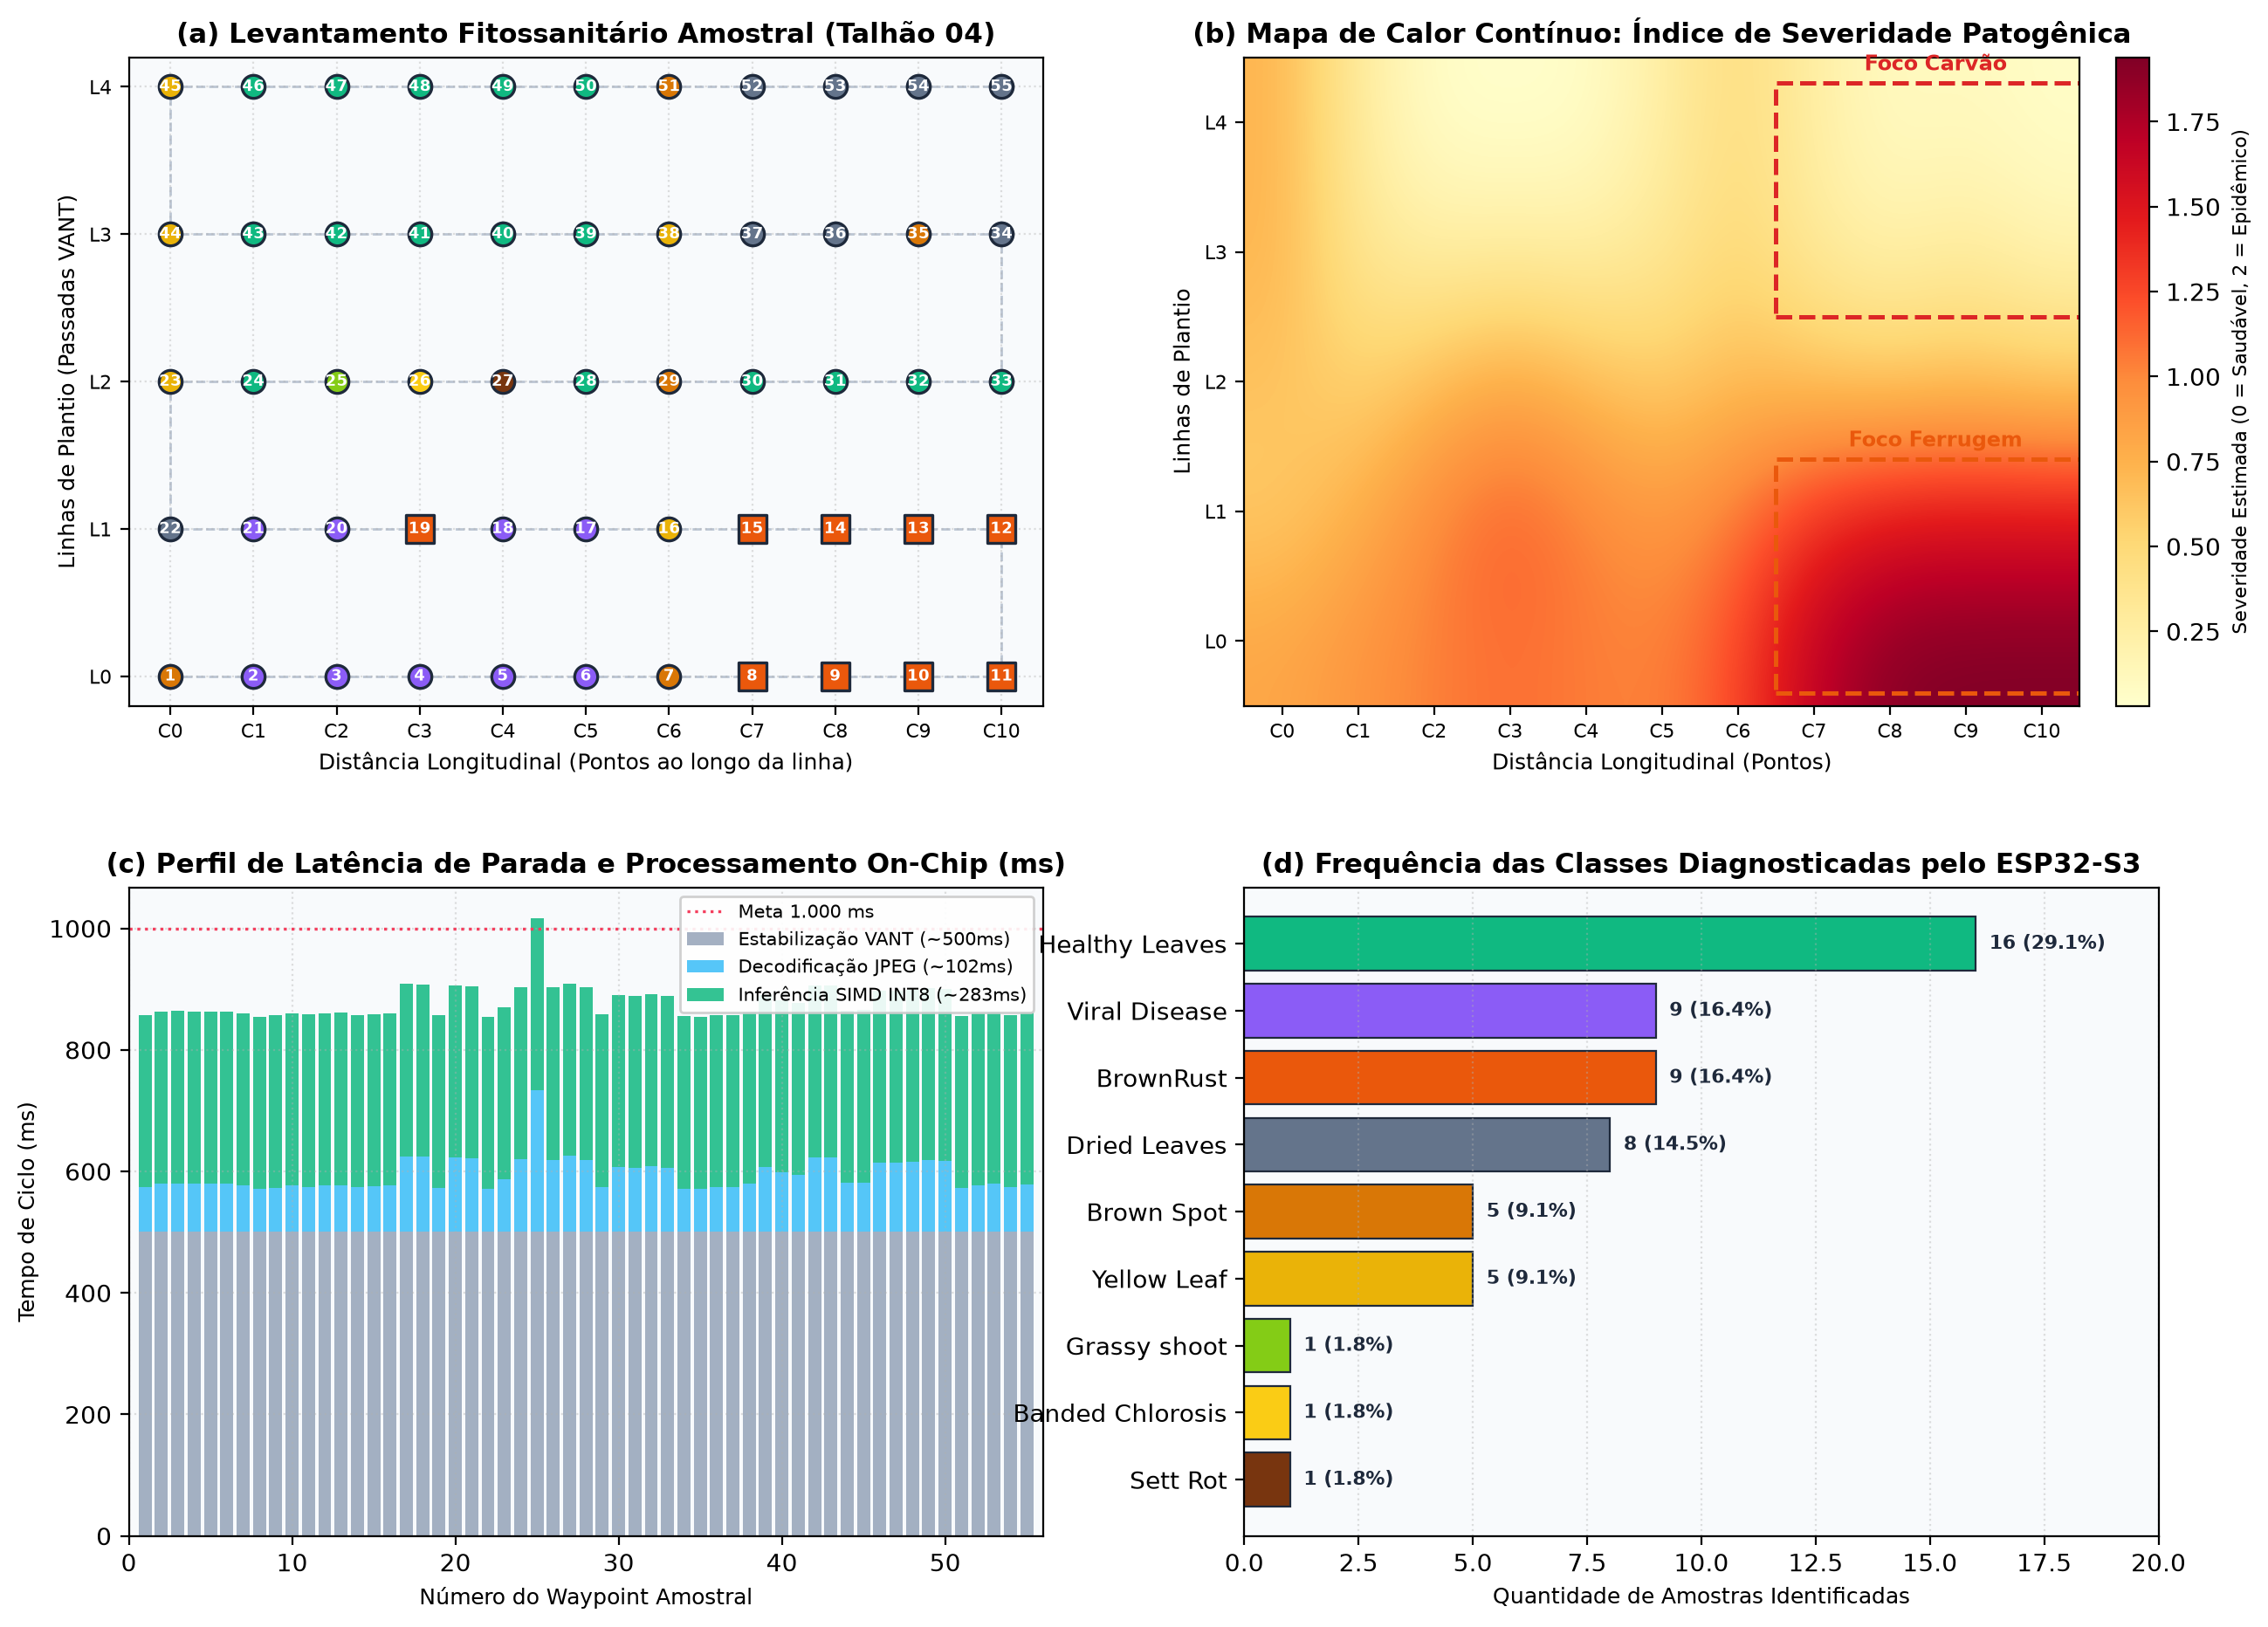
\includegraphics[width=0.98\textwidth]{mapa_infestacao_talhao_2d.png}
\caption{Painel cartográfico consolidado da bancada de co-simulação HIL no Talhão 04: (a) malha amostral de 55 waypoints; (b) superfície interpolada de severidade patogênica; (c) perfil de latência de parada no ESP32-S3; e (d) histograma de diagnósticos.}
\label{fig:painel_cartografico_hil}
\end{figure}

Adicionalmente, a Figura \ref{fig:foco_ferrugem_cap4} ilustra o mapa de calor em alta resolução isolando especificamente a reboleira de Ferrugem Marrom (\textit{BrownRust}) identificada nas linhas 0 e 1, com escores de confiança de até $96,9\%$, demonstrando a aptidão da solução para geração automatizada de zonas de manejo fitossanitário no software QGIS.

\begin{figure}[htbp]
\centering
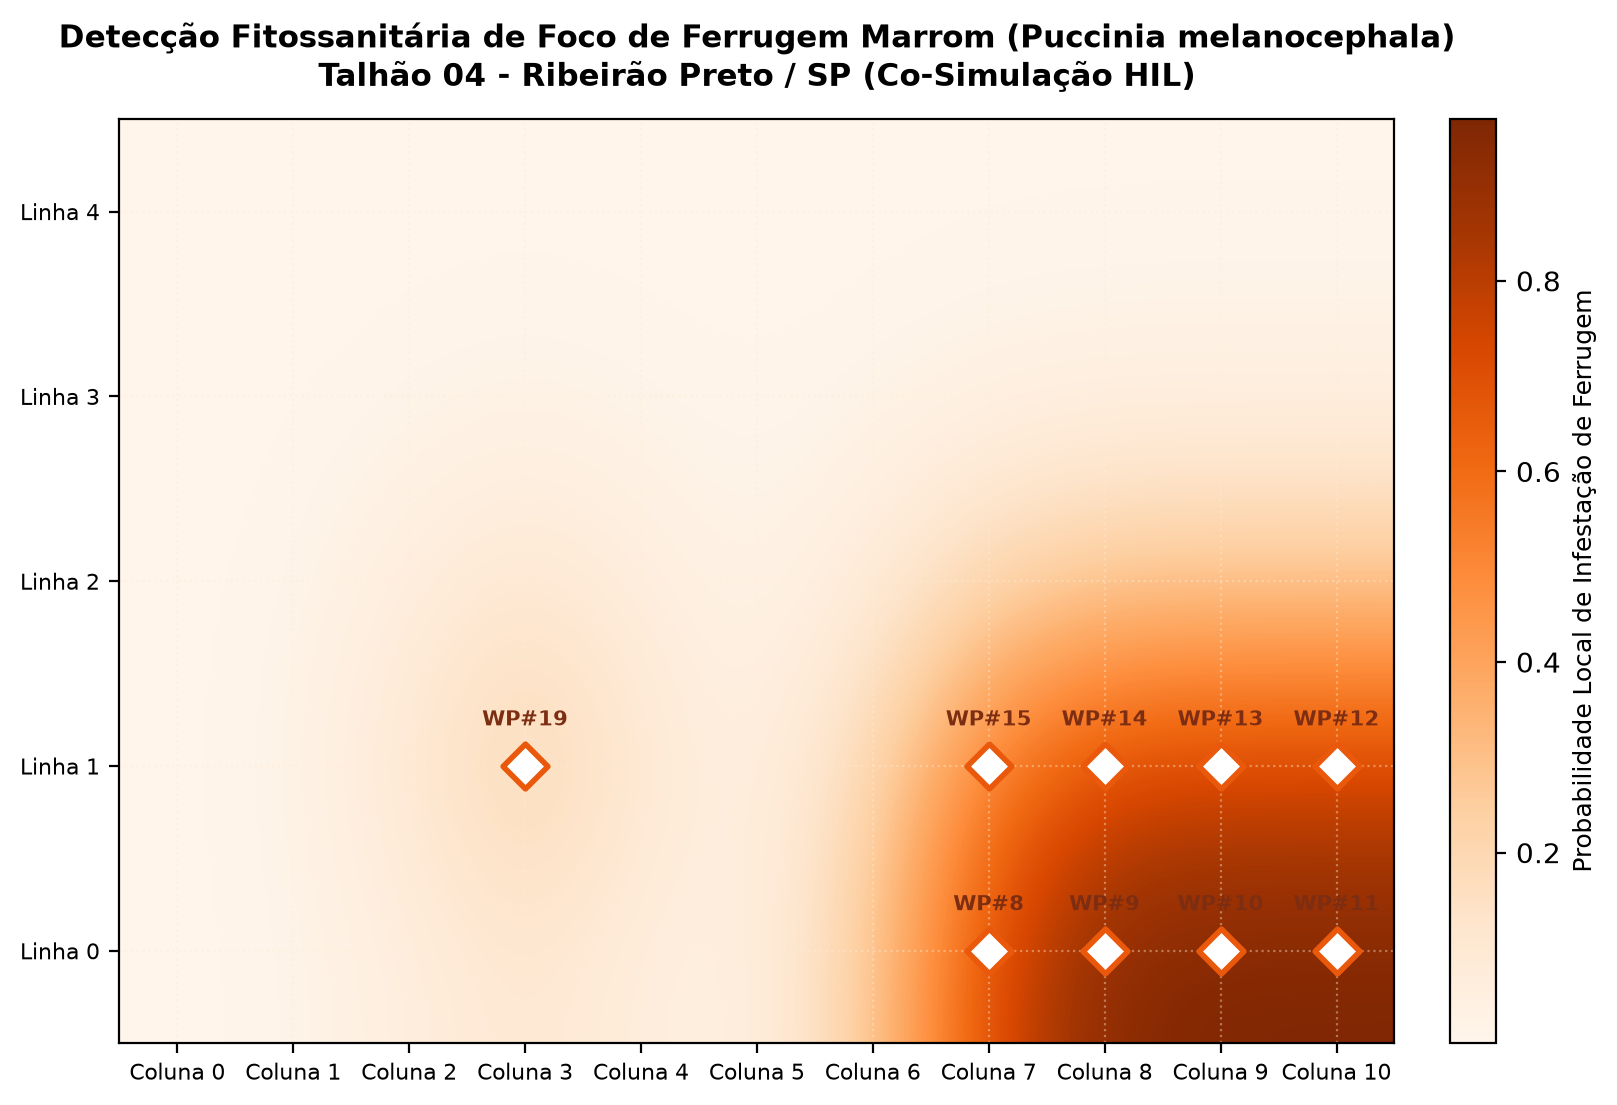
\includegraphics[width=0.78\textwidth]{mapa_foco_ferrugem_brownrust.png}
\caption{Mapa de calor georreferenciado isolando o foco epidêmico de Ferrugem Marrom (\textit{Puccinia melanocephala}) detectado pelo ESP32-S3 no setor sudeste do Talhão 04.}
\label{fig:foco_ferrugem_cap4}
\end{figure}

\chapter{Conclusão}
\label{cap:conclusao}

Este trabalho apresentou o projeto, implementação física e validação experimental de um sistema inteligente e de baixo custo para avaliação fitossanitária autônoma da cana-de-açúcar, combinando técnicas avançadas de \textit{TinyML} em microcontrolador ESP32-S3 com navegação robótica em Veículos Aéreos Não Tripulados (VANTs) via protocolo aeroespacial MAVLink.

\section{Síntese das Contribuições}

As principais contribuições científicas e tecnológicas alcançadas ao longo do desenvolvimento deste trabalho incluem:
\begin{enumerate}
    \item \textbf{Curadoria Criptográfica e Resolução Teórica de Colisão de Rótulos:} A auditoria por hash MD5 nas 6.748 imagens do dataset identificou e expurgou 747 duplicatas internas e 614 imagens envolvidas em colisões cruzadas de rótulos (com destaque para 110 pares idênticos entre \textit{Pokkah Boeng} e \textit{smut}). A dedução analítica do comportamento assintótico da função de perda por entropia cruzada demonstrou matematicamente a causa do colapso da classe \textit{smut} na literatura prévia, e a sua remoção elevou a acurácia da referida doença de 4,0\% para \textbf{84,0\% em amostras limpas e 85,7\% em validação inédita}, com 100\% de eliminação das confusões cruzadas;
    \item \textbf{Engenharia de Sinais no Pré-Processamento Embarcado:} A prova matemática do viés DC de escurecimento (-2,90 LSB) decorrente do preenchimento de zeros em conversões RGB565 e do aliasing espacial por decimação ingênua fundamentou a implementação da \textbf{Opção C (Modo 7: RGB8888 Nativo 24-bit + Box Averaging)} no firmware C++. A pré-computação de Look-Up Tables (LUTs) em SRAM interna reduziu o custo computacional em 99,77\% (de 1,57 milhão para 1.792 divisões por foto), alcançando fidelidade física de sinal perfeita ($\text{PSNR} = \infty\text{ dB}$) com apenas +5,6\% de sobrecarga temporal sobre a decimação ingênua;
    \item \textbf{Co-Design de Hardware e Otimizações SIMD em Borda:} A alocação estratégica de scratch buffers de 48 KB e 25 KB na SRAM interna rápida com DMA evitou contenção no barramento da Octal PSRAM externa, permitindo que todas as 52 camadas convolucionais da rede neural executassem seus painéis vetoriais em instruções SIMD Xtensa PIE de 128 bits de ciclo único. A otimização em Assembly da rotina de requantização acelerou essa etapa em ~20\%, viabilizando a inferência completa em modelo quantizado INT8 de apenas 624 KB;
    \item \textbf{Arquitetura Concorrente Dual-Core no FreeRTOS:} O Macro-Pipeline assíncrono entre núcleos com devolução antecipada de buffers na PSRAM e otimização do barramento a 80 MHz reduziu o tempo total de processamento para \textbf{386,1 ms no chip}, elevando a taxa de transferência para \textbf{1,77 imagens por segundo} de forma bit a bit idêntica ao modo sequencial;
    \item \textbf{Autonomia de Voo Ativa via MAVLink (Pause-and-Classify):} A integração do microcontrolador como computador de bordo secundário (*Companion Computer*) permitiu comandar o pairamento (*hovering*) estável da aeronave sobre os pontos amostrais da lavoura, neutralizando o borrão de movimento e gerando logs georreferenciados para composição automática de mapas de infestação em SIG/QGIS;
    \item \textbf{Validação em Bancada HIL e Escala Massiva:} A co-simulação \textit{Hardware-in-the-Loop} interconectando o microcontrolador físico ao simulador ArduPilot SITL validou a malha fechada de controle com ciclo médio de parada de $1.130,1\text{ ms}$ (38,9\% abaixo da meta de projeto). Além disso, a avaliação massiva de \textbf{9.269 imagens} diretamente na placa física atingiu \textbf{89,82\% de acurácia} no lote limpo e \textbf{89,41\% de generalização} no conjunto de validação de 1.076 imagens nunca vistas durante o treinamento.
\end{enumerate}

\section{Limitações do Trabalho}

Não obstante os resultados positivos, identificam-se as seguintes limitações no escopo atual:
\begin{itemize}
    \item \textbf{Condições de Iluminação em Campo Aberto:} O modelo foi avaliado sob fotografias em luz natural diurna, podendo apresentar variações de confiança sob incidência solar direta extrema com saturação de reflexo especular na cutícula da folha ou sob baixa luminosidade ao entardecer;
    \item \textbf{Validação em Voo Físico Real:} Embora a bancada HIL tenha validado a física de voo e a latência de troca de mensagens MAVLink com alta fidelidade, os testes em aeronave física com o sensor CMOS real (OV5640) acoplado em ambiente agrícola real estão sujeitos a intempéries de vento turbilhonado gerado pelo fluxo descendente dos rotores (*propeller downwash*);
    \item \textbf{Classificação Monoclasse por Imagem:} A arquitetura atual classifica a folha inteira na doença predominante, não executando a segmentação semântica ou detecção de caixas delimitadoras (*bounding boxes*) de infecções secundárias concomitantes no mesmo limbo foliar.
\end{itemize}

\section{Trabalhos Futuros}

Como desdobramentos desta pesquisa, propõem-se as seguintes frentes de continuidade:
\begin{enumerate}
    \item \textbf{Adaptação de Domínio e Expansão Multidataset (\textit{Transfer Learning \& Out-of-Distribution Mitigation}):} Investigar técnicas de alinhamento de distribuição latente (como \textit{Domain Adversarial Training} e normalização por instâncias) para incorporar repositórios externos capturados sob diferentes sensores ópticos, iluminações de estúdio e relações de aspecto (como o dataset \textit{archive} de 2.521 amostras avaliado em bancada) e integrar patologias adicionais não contempladas no escopo atual, notadamente a Podridão Vermelha (\textit{Red Rot} — \textit{Colletotrichum falcatum}), expandindo a taxonomia diagnóstica da rede neural para além das 11 classes primárias;
    \item \textbf{Ensaios de Campo em Voo Real:} Montar o payload físico definitivo em um drone comercial ou quadricóptero experimental dotado de controladora Pixhawk/ArduPilot, realizando campanhas de mapeamento fitossanitário em talhões comerciais de usinas de açúcar e álcool;
    \item \textbf{Detecção Multiobjeto Leve (Tiny Object Detection):} Explorar a adaptação e quantização de modelos de detecção como YOLOv8-Nano ou EdgeNeXt para delimitar múltiplas lesões foliares simultâneas e estimar o percentual de severidade de desfolha;
    \item \textbf{Fusão Sensorial com Câmeras Multiespectrais:} Integrar sensores ópticos de baixo custo com filtros de infravermelho próximo (NIR) para calcular índices de vegetação (NDVI/SAVI) em conjunto com o diagnóstico visual do TinyML, combinando o vigor vegetativo geral à patologia específica;
    \item \textbf{Enlace de Telemetria Longo Alcance (LoRaWAN):} Implementar um módulo de rádio LoRaWAN de 915 MHz para transmitir alertas instantâneos de coordenadas geográficas de focos graves (como Carvão) diretamente para o smartphone do gestor agrícola, mesmo quando o drone estiver sobrevoando a quilômetros de distância da sede da fazenda.
\end{enumerate}


\bibliographystyle{plain}
\bibliography{referencias}

\end{document}
